% !TeX root = ../../book.tex
\chapter[函数与基数]{函数与基数:输入、输出和集合的大小}\label{ch:chapter07}

% !TeX root = ../../../book.tex

\section{引言}

本章将继续探讨函数的第二部分内容。我们将正式给出函数的\emph{定义}。本质上,函数是具有特定性质的\textbf{关系}。这也解释了为何前期需要深入研究关系——不仅仅是因为关系本身具有的趣味性和实用性。定义函数后,我们将通过大量示例与证明,系统分析函数可能具备的各种性质。在此过程中,我们将综合运用先前所学的全部概念,特别是 \ref{sec:section4.9} 节中的证明技巧。

本章后半部分将引入\emph{双射函数} (Bijective Function) 的概念,即集合间元素的一一对应关系,用以讨论集合的``大小''及其比较方法。该主题称为\emph{基数} (Cardinality),它将揭示无限集领域中若干惊人且反直觉的结论。这也为下一章关于有限集及其计数方法的研究奠定基础。

% !TeX root = ../../../book.tex

\subsection{目标}

以下简短内容将向你展示本章如何融入本书的体系。我们会解释之前的工作对本章研究的帮助,说明我们为什么要探讨本章的主题,并告诉你我们的目标以及在阅读时需要注意的事项。现在,我们将通过几条陈述总结本章的主要目标。这些陈述概括了你在完成本章后应掌握的技能和知识。接下来的章节会更详细地解释这些思想,这里仅提供一个简要列表供你参考。完成本章后,请返回这个列表,检查你是否理解所有目标。你能看出我们为什么认为这些目标重要吗?你能解释我们使用的术语并应用我们描述的技术吗?

\textbf{学完本章后,你应该能够……}

\begin{itemize}
    \item 定义函数,并提供多个例子。
    \item 使用函数的非正式描述和可视化图像来构建关于函数(示例和反例)及其属性的正式论证。
    \item 在函数的上下文中定义集合的像 (Image) 和原像 (Pre-image),并证明这些操作的各种属性。
    \item 陈述函数的属性,并应用相关方法来确定和证明给定函数是否具有这些属性。
    \item 找出两个函数的复合,说明如何用它们来创建新函数,并解释和证明复合对所涉及函数属性的影响。
    \item 描述双射函数 (Bijective Function) 和反函数 (Inverse Function) 之间的关系,并用它们来解决问题和证明结论。
    \item 使用双射来定义集合的基数 (Cardinality),并证明关于这些基数的结论。
    \item 说明有限集、可数无限集和不可数无限集之间的区别,并提供每种类型的多个例子。
\end{itemize}

% !TeX root = ../../../book.tex

\subsection{承上}

前一章介绍的重要概念\textbf{关系}将在本章发挥核心作用。我们已经指出\textbf{函数}实际上是一种特殊的关系,这一点将在其正式定义中得以体现。

至于前一章讨论的其他概念(如等价关系及数论相关结论),本章不会直接涉及。换言之,本章对函数及其性质的探讨不依赖于这些概念,但我们将运用它们设计若干启发性示例与练习。

% !TeX root = ../../../book.tex

\subsection{启下}

正如前一章所述,你可能已经通过数学课程或编程实践对函数有了一定直观理解。我们始终强调要以严谨的\emph{数学语言}定义研究对象,函数自然也不例外!形式化定义将帮助我们精准描述那些既往难以言明的函数性质。此外,函数的特定性质还将为后续探讨集合的\emph{基数}奠定基础——请相信我,如果不深入掌握函数理论,便无法真正进入这一主题。


% !TeX root = ../../../book.tex

\subsection{忠告}

我们还要重申上一章中的一些忠告和建议。我们正在继续探索一些抽象的数学领域。本章特别是要将一个你可能在视觉和直觉上熟悉的概念放在更严格的基础之上。我们会尽可能利用大家的直觉,但也无法避免地需要进行抽象思维和问题解决的过程。特别是,我们无法总是将函数与它的图像联系起来,尽管这是我们在数学学习早期常用且有效的方法。此外,在基数的讨论中,我们会遇到一些完全违反直觉的结果。真的!这些奇怪又反直觉的事实需要我们保持开放的心态去理解。

\newpage
% !TeX root = ../../../book.tex
\section{定义与示例}

你一般如何理解函数?对函数的直观印象是什么?能否用数学对象严格\emph{定义}函数?不妨尝试一下!运用已学的概念和工具,能否仅用这些内容表达你对\emph{函数}的理解?请先认真思考,再阅读下文。我们将逐步建立函数的定义,之后你再尝试自行定义。

我们通常将函数视为一种\emph{规则}或\emph{映射},用于为每个输入指定唯一输出。例如定义在 $\mathbb{R}$ 上的函数 $f(x) = x^2$,它接受一个实数并输出其平方。函数 $f$ 如同一台``机器'',将数字转化为其平方;``在 $\mathbb{R}$ 上''表明仅允许输入实数。但如何确定机器允许的输出范围呢?这里暴露了直观解释的缺陷:理想情况下,定义函数时需要明确三要素——输入范围、输出范围(未必是所有可能的输出,也可以是输出的对象类型)以及对应``规则''。如果把函数视为\emph{映射},则它就像描述集合间的``路径''(如平方运算),从输入集($\mathbb{R}$)导向输出集($\mathbb{R}$)。在这种解释中,仍然需要完整传达上述信息,但也提供了新视角。

在给出定义之前,先来思考一个问题:假设有一个``规则'',它的输入是人,输出是这个人的眼睛颜色,你会如何将其表示为 $f(x) = \dots$ 的形式呢?这极其困难!几乎需要完整复述语句才能定义``规则''。其输入/输出既非实数也非整数,而是全新对象。然而此类函数却是合理的,理应被定义涵盖。试着比较该函数与实数集 $\mathbb{R}$ 上 $f(x) = x^2$ 的异同(或并无本质区别)。

(你甚至可能会反驳说这根本就不是一个\emph{函数}!万一某人两只眼睛异色呢?此时``映射''的输出又是什么?此问题值得深究!)

好了,现在轮到你了。试着用前几章讨论过的概念、术语和数学对象自行定义\emph{函数}。

% !TeX root = ../../../book.tex

\subsection{定义}

我们将使用以下定义。或许它与你的定义接近,甚至相同,或者只是措辞略有不同。但这个定义完美地概括了我们前面对函数的直观概念(将函数看作一种分配\emph{规则}),并用我们一直以来在发展的集合和逻辑语言来表达。这样做有几个好处:

\begin{enumerate}[label=(\alph*)]
    \item 它为函数提供了严格的基础,使我们能够在数学意义上放心地使用它们;
    \item 它让我们能够讨论函数的性质,并用数学术语和概念来证明这些性质;
    \item 它使我们能够概括函数的概念,并将其应用于比我们熟悉的标准数集更抽象的场景中。
\end{enumerate}
好了,解释到此为止,我们来看定义。\\

\begin{definition}
    设 $A, B$ 为集合。设 $f$ 为 $A, B$ 间的关系,所以 $f \subseteq A \times B$。同时假设 $f$ 具有如下性质:
    \[\forall a \in A \centerdot \exists! b \in B \centerdot (a, b) \in f\]
    (回想一下,``$\exists!$'' 表示``存在唯一的……'',也就是说``有且只有一个……'')

    这样的关系称为 $A$ 到 $B$ 的 \dotuline{函数}。

    我们称 $A$ 为函数的\dotuline{定义域},$B$ 为函数的\dotuline{值域}。

    写做
    \[f:A \to B\]
    表示 $f$ 是 $A$ 到 $B$ 的函数。

    如果 $(a,b) \in f$,则我们写做
    \[f(a) = b\]
    并且知道对于给定的 $a$,$b$ 是唯一满足该属性的元素。
\end{definition}

就是这样!虽然现在把\emph{函数}看作一种\emph{关系} --- 实际上是一种特殊的\emph{集合} --- 可能有点奇怪,但这正是它的本质。用这种方式定义函数让我们能够用集合和关系的语言来讨论它们,同时我们仍然可以使用一些熟悉的符号。对于每一个``输入'' $a$(即\emph{定义域}中的每一个元素),都有\emph{唯一}一个``输出'' $b$(即\emph{值域}中的一个元素)。因此,我们可以写成 $f(a) = b$,并且知道 ``$=$'' 表示真正的相等关系,因为只有这个唯一的 $b$ 满足这种关系。

这种定义的一部分包含了我们之前提到的想法:我们想知道函数会``输出''什么\emph{类型}的对象。这就是通过指定值域实现的。例如,定义函数 $f : \mathbb{R} \to \mathbb{R}$ 为 $f(x) = \sqrt{x}$ 是不合适的,因为定义域中的某些元素(即负数)会使``输出''未定义。(技术上讲,输出会是一个复数,而复数不是值域 $\mathbb{R}$ 的元素;在 $\mathbb{R}$ 的上下文中,我们认为复数是``未定义''的。)当一个函数被正确定义,且定义域和值域已明确,并且相关的对确实属于集合的笛卡尔积时,我们称这个函数是\textbf{良好定义的}。有时,我们会给出两个集合之间的关系,并要求你判断它是否是\emph{良好定义的函数}。实际上,这就是在问这个关系是否符合函数的定义。

\subsubsection*{范围}

\emph{值域}这个词对你来说可能比较陌生。实际上,你可能更习惯用\textbf{范围}来指代函数的\emph{潜在}``输出''集合。我们想在这个上下文中完全避免使用``范围''一词,因为它可能会产生歧义。有些作者和老师用``范围''来表示我们这里所说的``值域'',即函数的\emph{潜在}``输出''集合;而另一些人则用它来表示本书所说的``像'',即函数的\emph{实际}``输出''集合。在 \ref{sec:section7.3} 节中我们会详细定义这个术语。通常,像是值域的子集,但往往可能是\emph{真}子集。当有人使用``范围''这个词时,他们可能指的是这两种解释中的其中一个,而你可能理解的是另一个!为了避免这种混淆,我们将只使用\emph{值域}和\emph{像}这两个词。

% !TeX root = ../../../book.tex

\subsection{示例}

让我们使用新的定义来看几个函数(以及非函数)的例子。在处理这些例子时,我们将介绍定义和使用函数的正确符号,并描述如何``可视化''某些函数,以便更好地理解它们。

\subsubsection*{符号}

有几种正确定义函数的方法。以下都是定义``实数平方函数''的正确方法:
\begin{quotation}
    定义函数 $f \subseteq \mathbb{R} \times \mathbb{R}$ 为 $(x, y) \in f \iff y = x^2$。

    定义函数 $f : \mathbb{R} \to \mathbb{R}$ 为 $f=\big\{(x,x^2) \mid x \in \mathbb{R}\big\}$。

    定义函数 $f : \mathbb{R} \to \mathbb{R}$ 为 $\forall x \in \mathbb{R} \centerdot f(x) = x^2$。
\end{quotation}
考虑每种方法为什么符合我们上面给出的函数定义。第一种方法直接表明函数是一种\emph{集合},即从 $\mathbb{R}$ 到 $\mathbb{R}$ 的关系。第二种方法使用相同的概念,但通过集合构建符来表示 $f$,而不是用\emph{充要条件}语句。第三种方法表明每个 $f$ 的``输入''都有\emph{唯一}一个``输出'',所以我们可以简单地声明\emph{对于所有} $x \in \mathbb{R}$ 的``输出''。

我们\emph{通常}会坚持使用第三种符号风格,因为它更容易理解,并且更符合我们对函数的直观认识。有时,我们也会使用其他符号风格;例如,我们想要强调函数的底层结构,或者仅仅可能是为了更容易书写。不过,一般来说,在定义函数时,我们需要为读者明确所有重要的组成部分:\emph{定义域}、\emph{值域}、\emph{函数名},以及分配有序对的\emph{规则}或\emph{集合}。

如果你在想为什么在定义函数时指定\emph{值域}如此重要,可以从编写计算机代码的角度来考虑。当你定义一个函数时,通常需要\emph{声明}输出变量的数据类型。(当然,这也取决于具体的编程语言。)以 \verb|Java| 为例,你可能会写
\begin{verbatim}
    public int PlusOne (int x) {
        return x+1;
    }
\end{verbatim}
上面代码定义了一个函数,它输入一个整数,加一后输出另一个整数。请注意,你必须告诉程序输入的数据类型是什么以及输出的数据类型是什么。\\

\begin{example}
    考虑一个将自然数转换为其二进制表示的函数。我们用 $B$ 表示这个函数。通过计算,我们希望 $B(1) = 1, B(2) = 10, B(10) = 1010$。那么,这个函数的定义域是什么?值域是什么?你能严格地写出它的定义\emph{规则}吗?还是用文字描述更好呢?

    我们可以这样定义这个函数。设 $S$ 为所有由 $0$ 和 $1$ 组成的有限二进制字符串的集合。然后定义函数 $B : \mathbb{N} \to S$ 为
    \[B = \{(n, s) \mid n \in \mathbb{N} \;\text{且}\; s \;\text{为}\; n \;\text{的二进制表示}\}\]
\end{example}

\begin{example}
    再次考虑``平方函数'':设 $f : \mathbb{R} \to \mathbb{R}$ 定义为 $\forall x \in \mathbb{R}, f(x) = x^2$。这函数与下面的函数有区别吗?
    \begin{itemize}
        \item 设函数 $g : \mathbb{R} \to \mathbb{C}$ 定义为
            \[\forall x \in \mathbb{R} \centerdot g(x) = x^2\]
        \item 设函数 $h : \mathbb{Z} \to \mathbb{R}$ 定义为
            \[\forall x \in \mathbb{Z} \centerdot h(x) = x^2\]
    \end{itemize}

    函数 $g$ 的值域不同,但实际上,$\mathbb{R} \subseteq \mathbb{C}$。所有有序对 $(x, x^2) \in g$ 仍然满足 $x \in \mathbb{R}$ 且 $x^2 \in \mathbb{R}$。从这个角度来看,$f$ 和 $g$ 是\emph{相同的}函数,我们可以写做 $f = g$。稍后,我们将详细探讨两个函数相等的确切含义。目前,只需说明 $f$ 和 $g$ 对应的底层关系具有相同的实数有序对作为元素即可。理论上,函数 $g$ \emph{允许}第二个值为复数,但由于定义域和``规则''的设定,这实际上不会发生。

    函数 $h$ 的定义域不同,并且 $\mathbb{Z} \subset \mathbb{R}$(是 $\mathbb{R}$ 的真子集)。因此,在函数 $f$ 对应的关系中,有许多有序对并不属于函数 $h$ 对应的关系。例如,$(\frac{1}{2}, \frac{1}{4}) \in f$ 但 $(\frac{1}{2}, \frac{1}{4}) \notin h$。换句话说,$f(\frac{1}{2}) = \frac{1}{4}$,但 $h(\frac{1}{2})$ 的概念没有\emph{良好定义},因为 $\frac{1}{2}$ 不属于 $h$ 的定义域。
\end{example}

\begin{example}
    我们也可以\textbf{分段}定义函数。例如,考虑定义在 $\mathbb{R}$ 上的\emph{绝对值函数}:

    设函数 $a : \mathbb{R} \to \mathbb{R}$ 定义为
    \[\forall x \in \mathbb{R} \centerdot a(x) = 
    \begin{cases}
         x &\text{如果}\; x \ge 0 \\
        -x &\text{如果}\; x < 0
     \end{cases}\]
     定义域中的每个元素都\emph{恰好}落入某一种情况,因此没有歧义。
\end{example}

\subsubsection*{``良好定义的''函数}

我们并不总是能明确一个定义的关系是否真正是一个函数。面对一个给定的定义域、值域和一个``规则''或集合,我们该如何验证它们是否构成一个函数呢?接下来我们将给出一个定义(完全基于之前讨论的函数定义)来解决这个问题:

\begin{definition}\label{def:definition7.2.5}
    给定定义域 $A$、值域 $B$ 和``规则'' $f$,我们说 $f$ 是一个\dotuline{良好定义的函数},当且仅当
    \begin{enumerate}[label=(\arabic*)]
        \item 该规则定义在 $A$ 的所有元素上;
        \item 对于每个 $a \in A$,该规则都输出集合 $B$ 中的唯一一个元素。
    \end{enumerate}
\end{definition}

让我们用一个例子来说明这个概念。在本节的后面,我们还会看到一些不是函数的例子,并且会再次引用这个\textbf{良好定义的函数}的定义。\\

\begin{example}
    设函数 $a : \mathbb{Z} \to \mathbb{N}$ 定义为
    \[\forall z \in \mathbb{Z} \centerdot f(z) = |2z + 1|\]
    等一下,我们怎么确定对于任意\emph{整数} $z$,$|2z + 1|$ 为\emph{自然数}?这不是那么显然,但我们可以证明出来。

    假设 $z \in \mathbb{Z}$ 满足 $z \ge 1$。则 $2z+1 \in \mathbb{Z}$ 且 $|2z+1| = 2z+1 \ge 3$。因此 $f(x) \in \mathbb{N}$。

    假设 $z \in \mathbb{Z}$ 满足 $z \le -1$。则 $2z+1 \in \mathbb{Z}$ 且 $2z+1 \le -1$。因此 $f(x) = |2z + 1| ≥ 1 \in \mathbb{N}$。所以 $f(x) \in \mathbb{N}$。

    假设 $z = 0$。则 $f(z) = |2 \cdot 0 + 1| = 1$,所以 $f(z) \in \mathbb{N}$。

    无论哪种情况,我们发现定义函数 $f$ 的``规则''确实会生成一个自然数,这个数是\emph{值域}中的元素。而且,它只生成这样一个数。因此,这是一个良好定义的函数。
\end{example}

\begin{example}
    设 $P$ 为世上所有人的集合。函数 $b : P \to \mathbb{N} \cup \{0\}$ 定义为
    \[b = \{(p, n) \mid p \in P \land p \;\text{有}\; n ;\text{个姐妹}\}\]
    (请注意,为了练习,我们这里使用了一种强调集合的符号风格。另外,将数学符号和文字结合起来可能看起来有些奇怪,例如 ``$b(p) = p \;\text{这个人有多少个姐妹}$''。)

    这是一个良好定义的函数吗?我们认为是的。假如你走到某人面前(即某个元素 $p \in P$),问他们有多少姐妹(即 $b(p)$ 的值)。他们会告诉你一个非负整数,并且他们不可能给出两个\emph{不同的}数字。

    现在,你可能会指出,在今天这个离婚和再婚普遍的社会中,很多人有\emph{同父异母或同母异父的姐妹} (half-sisters),而 $\frac{1}{2} \notin \mathbb{N} \cup \{0\}$。这个观点很合理。但是,在``简化假设''下,即假设每个人都有\emph{整数数量}的姐妹,这个函数是良好定义的。
\end{example}

\subsubsection*{恒等函数}

\begin{example}
    设 $S$ 为集合。是否\emph{必然}存在一个从 $S$ 到 $S$ 的函数?当然,我们可以想到许多从 $\mathbb{R}$ 到 $\mathbb{R}$ 的函数,但如果 $S$ 只是某个任意集合呢?我们能保证存在一个从 $S$ 到 $S$ 的函数吗?事实证明……是的,我们可以!回想一下我们在讨论关系时曾考虑过的一个类似问题(参见示例 \ref{ex:example6.2.9})。我们知道在集合 $S$ 上我们总是可以定义\emph{等价关系};也就是说,我们可以通过 $(x, y) \in R \iff x = y$ 在 $S$ 上定义 $R$。对于每个 $x \in S$,这个关系由所有形式为 $(x, x)$ 的有序对组成。这个关系是否表示一个函数?我们只需检查定义属性:每个输入是否只有一个输出?看起来确实如此!集合中的任意元素只等于它自己,而不等于其他任何元素。因此,$R$ 确实表示一个函数。这是一个特别的函数,我们给它起了一个特定的名字。
\end{example}

\begin{definition}
    设 $S$ 为集合。$S$ 上的\dotuline{恒等函数}为函数 $Id : S \to S$ 定义为
    \[\forall x \in S \centerdot Id(x) = x\]
\end{definition}

也就是说,恒等函数``输出与输入完全相同''。(可以把函数想象成一台机器,这台懒惰的机器什么也不做,只是原样输出输入的内容。)

有时,我们需要引用在\emph{不同}集合上定义的恒等函数。为避免混淆,我们用 $Id_S$ 表示``\textbf{集合 $S$ 上的}恒等函数''。

\subsubsection*{不是函数的例子}

有时候,在解决问题时,我们可能会提出一个关于两个集合之间的``规则'',并想知道它是否是一个函数。也许我们需要它是一个函数来帮助我们解决问题。那么,这个规则在什么情况下可能不成立呢?换句话说,我们可以通过什么来证明一个提出的规则不是一个函数呢?回顾一下\textbf{良好定义的函数}的定义(见定义 \ref{def:definition7.2.5}),有三种不同的情况可能出错:

\begin{itemize}
    \item 可能存在某个定义域中的元素\textbf{没有对应的``输出''}。
    \item 可能存在某个定义域中的元素\textbf{有多个``输出''}。
    \item 可能存在某个定义域中的元素只有一个``输出'',但该``输出''\textbf{不在值域中}。
\end{itemize}
以下例子说明了这些情况。\\

\begin{example}
    设函数 $G : \mathbb{N} \times \mathbb{N} \to \mathbb{N}$ 定义为
    \[\forall (a, b) \in \mathbb{N} \times \mathbb{N} \centerdot G(a, b) = a - b\]
    这\textbf{不是}一个良好定义的函数,因为有定义域中的很多元素其输出不在值域中。例如,$(5, 10) \in \mathbb{N} \times \mathbb{N}$ 且 $G(5, 10) = -5$,但 $-5 \notin \mathbb{N}$。
\end{example}

\begin{example}
    假设 $W$ 为所有英语单词的集合。定义 $A: W \to W$ 为输入一个单词并输出一个不是原单词的异序词 (anagram)\footnote{异序词 (anagram) 指的字母相同但顺序不同的单词}。这\textbf{不是一个良好定义的}函数,原因有几个。例如,$A(\text{HI})$ 和 $A(\text{FUNCTION})$ 都不存在。此外,像 $A(\text{INTEGRAL})$ 这样的单词有多个(即非唯一的)输出:TRIANGLE, ALERTING, ALTERING……。
\end{example}

% !TeX root = ../../../book.tex

\subsection{函数相等}

有时候,两种函数虽然由不同的规则或公式定义,但实际上它们对应相同的底层关系!在这种情况下,这两个函数是\textbf{相等的}。我们将先用函数符号来描述这种情况,然后再用底层关系和集合符号来证明这一点。

两个函数如何才能\emph{相等}呢?首先,它们的定义域必须相同。如果定义域不同,那么其中一个定义域中包含了另一个定义域中没有的元素,这就会出现问题。(想象一下:一个函数在某个元素上有定义,而另一个函数在相同元素上没有定义,这样它们就不可能相等)。假设我们有两个集合 $A$ 和 $B$,以及两个函数 $f : A \to B$ 和 $g : A \to B$。为了使 $f$ 和 $g$ 相等,我们需要满足什么条件呢?函数的定义特征是,对于任意输入 $x \in A$,函数 $f$ 和 $g$ 都有\emph{唯一}的输出 $f(x)$ 和 $g(x)$。如果 $f$ 和 $g$ 是相同的函数,那么我们必有 $f(x) = g(x)$!这让我们可以陈述以下定理。

\begin{theorem}
    设 $A, B$ 为集合。并设 $f : A \to B$ 和 $g : A \to B$ 为函数。假设
    \[\forall x \in A \centerdot f(x) = g(x)\]
    则我们称 $f$ 和 $g$ 是相等的函数,记作 $f = g$。
\end{theorem}

这确实是一个\emph{定理}。这个想法虽然非常直观,但它并没有在函数的\emph{定义}中明确提到。因此,我们必须证明这个想法。为了解释这一点,我们将考虑属于关系 $f$ 和 $g$ 的所有有序对。通过证明这些有序对是相同的,我们可以在集合意义上得出 $f = g$。请注意,我们将进行\emph{双重包含}论证!

\begin{proof}
    设 $A, B$ 为集合。并设 $f : A \to B$ 和 $g : A \to B$ 为函数。假设
    \[\forall x \in A \centerdot f(x) = g(x)\]

    首先,我们证明 $f \subseteq g$。给定 $(a,b) \in f$。因为 $f$ 为函数,这意味着 $f(a) = b$。根据主假设,可得 $f(a) = g(a)$,所以 $g(a) = b$。因此 $(a,b) \in g$。这表明
    \[(a, b) \in f \implies (a, b) \in g\]
    因此 $f \subseteq g$。

    接着,我们用相同的方法证明 $g \subseteq f$。给定 $(c,d) \in g$。因为 $g$ 为函数,这意味着 $g(c) = d$。根据主假设,可得 $f(c) = g(c)$,所以 $f(c) = d$。因此 $(c,d) \in f$。这表明
    \[(c, d) \in g \implies (c, d) \in f\]
    因此 $g \subseteq f$。

    由于我们已经证明了 $f \subseteq g$ 和 $g \subseteq f$,我们可以得出结论 $f = g$。
\end{proof}

这为我们提供了一种简便的方法来证明两个函数相等,而不需要深入探讨它们的底层关系或集合结构。我们只需要证明两个函数对于定义域中的每一个元素,其输出是相同的。接下来,我们通过几个例子来说明这一点。\\

\begin{example}
    设 $A = \{-1, 0, 1\}$。定义函数 $f_1 : A \to \mathbb{Z}$ 和 $f_2 : A \to \mathbb{Z}$ 为
    \[\forall x \in A \centerdot \big(f_1(x) = x\big) \land \big(f_2(x) = x^3\big)\]
    我们来证明 $f_1 = f_2$。由于定义域只包含三个元素,我们可以逐一检验输出。
    \begin{align*}
        f_1(-1) = -1 &= (-1)^3 = f_2(-1)\\
        f_1(0) = 0 &= 0^3 = f_2(0)\\
        f_1(1) = 1 &= 1^3 = f_2(1)
    \end{align*}
    因此,对于每一个合法输入(即 $\forall x \in A$)函数 $f_1$ 和 $f_2$ 有相同的输出(即 $f_1(x) = f_2(x)$)。因此 $f_1 = f_2$。
\end{example}

\begin{example}
    设 $B = \{1, 2, 3\}$。定义函数 $g_1 : B \to \mathbb{Z}$ 和 $g_2 : B \to \mathbb{Z}$ 为
    \[\forall n \in B \centerdot \big(g_1(n) = n^3-n^2-6\big) \land \big(g_2(n) = 5n^2-11n\big)\]
    我们来证明 $g_1 = g_2$。定义域还是只有三个元素,所以我们可以手工检验所有相等性。
    \begin{align*}
        g_1(1) &= 1^3 - 1^2 - 6 = 1 - 1 - 6 = -6 \\
        g_2(1) &= 5 \cdot 1^2 - 11 \cdot 1 = 5 - 11 = -6 \\
        \\
        g_1(2) &= 2^3 - 2^2 - 6 = 8 - 4 - 6 = -2 \\
        g_2(2) &= 5 \cdot 2^2 - 11 \cdot 2 = 20 - 22 = -2\\
        \\
        g_1(3) &= 3^3 - 3^2 - 6 = 27 - 9 - 6 = 12 \\
        g_2(3) &= 5 \cdot 3^2 - 11 \cdot 3 = 45 - 33 = 12
    \end{align*}
    因此 $\forall n \in B \centerdot g_1(n) = g_2(n)$,所以 $g_1 = g_2$。
\end{example}

由于这两个例子的定义域都较小,我们可以逐一检查每个元素。然而,并不是所有情况都是如此。有时,我们需要考虑定义域内的任意元素(因为我们要证明的性质是以 ``$\forall$'' 量词开头的),并基于此进行分析。实际上,这个例子有一种有趣的方法可以实现这一点,现在我们就来展示一下它是如何实现的。

给定 $n \in B$。由于 $g_1(n)$ 和 $g_2(n)$ 都属于 $\mathbb{Z}$,我们可以考虑它们的差。具体来说,我们发现
\begin{align*}
    g_1(n) - g_2(n) &= (n^3 - n^2 - 6) - (5n^2 - 11n) \\
    &= n^3 - 6n^2 - 11n - 6 \\
    &= (n - 1)(n - 2)(n - 3)
\end{align*}
(注意:读者可以通过简单地展开这三项的乘积来验证最后的等式。)

由于 $n \in B$,我们知道 $n$ 可能是 $1,2,3$。在每种情况下,其中一项 --- $(n - 1), (n - 2), (n - 3)$ --- 必定为零。因此
\[g_1(n) - g_2(n) = (n - 1)(n - 2)(n - 3) = 0\]
据此,我们得到 $g_1(n) = g_2(n)$。由于这对任意 $n \in B$ 都成立,我们可以得出结论 $g_1 = g_2$。

我们要指出,这比在这个特定例子中``检查所有情况''的方法要复杂得多。我们是怎么知道要关注差的呢?我们又是怎么知道它会这样分解的呢?这正是数学的魅力所在!我们可能通过思考如何解决一个更普遍的问题来找到这种巧妙的方法,因为在这种情况下,定义域太大,根本无法逐一考察每个案例。我们可能会识别出因式分解,或者从 $B = \{1, 2, 3\}$ 这个事实中猜到它。如果你仔细思考,你可能会明白我们是如何想出这个例子的!$\smiley{}$

让我们来看一个更复杂的函数相等的例子。它涉及一些我们假设你不熟悉的概念,我们也不会再次讨论它们,但我们认为这个例子足够有趣和有启发性,所以将其呈现在这里。\\

\begin{example}
    我们将在这里定义两个函数,并说明它们为何相等。设每个函数的定义域和值域为 $\mathbb{R}^2$(实平面)。现在,让我们通过几何方式(即视觉上)来定义两个函数 $F_1$ 和 $F_2$。我们希望 $F_1$ 输入平面上的一个点 $p$,并输出将 $p$ 围绕原点逆时针旋转 $90 \degree$ 后再根据原点镜像得到的点。而 $F_2$ 则是输入点 $p$,并输出将 $p$ 顺时针旋转 $90 \degree$ 后得到的点。为了更好地理解这两个函数的含义,请看以下 $F_1$ 和 $F_2$ 在特定点上的示意图。

    \begin{multicols}{2}
        \begin{center}
            {\begin{tikzpicture}
                \draw[latex-latex] (-3,0) -- (3,0); 
                \draw[latex-latex] (0,-3) -- (0,3); 
                \draw (0,0) -- (1.5,1.5);
                \node at (1.5, 1.5)[circle,fill,inner sep=2pt]{};
                \draw[shift={(1.6, 1.5)}] node[right] {$p$};
                \draw (0,0) -- (-1.5,1.5);
                \node at (-1.5, 1.5)[circle,fill,inner sep=2pt]{};
                \draw[rotate=45] (0,0) rectangle (0.3,0.3);
                \draw (0,0) -- (1.5,-1.5);
                \node at (1.5, -1.5)[circle,fill,inner sep=2pt]{};
                \draw[shift={(1.6, -1.7)}] node[right] {$F_1(p)$};
                \draw[dashed,-latex] (1.5, 1.5) .. controls (0.5, 2.8) and (-0.5, 2.8) .. (-1.4, 1.6);
                \draw[shift={(-0.5, 2.6)}] node[left] {\small 旋转 $90 \degree$};
                \draw[dashed,-latex] (-1.5, 1.5) .. controls (-2, 0) and (-1.5, -2) .. (1.4, -1.6);
                \draw[shift={(-1.0, -0.3)}] node[right] {\small 围绕};
                \draw[shift={(-1.0, -0.7)}] node[right] {\small 原点};
                \draw[shift={(-1.0, -1.1)}] node[right] {\small 镜像};
            \end{tikzpicture}}
        \end{center}

        \begin{center}
            {\begin{tikzpicture}
                \draw[latex-latex] (-3,0) -- (3,0); 
                \draw[latex-latex] (0,-3) -- (0,3); 
                \draw (0,0) -- (1.5,1.5);
                \node at (1.5, 1.5)[circle,fill,inner sep=2pt]{};
                \draw[shift={(1.6, 1.5)}] node[right] {$p$};
                \draw (0,0) -- (1.5,-1.5);
                \node at (1.5, -1.5)[circle,fill,inner sep=2pt]{};
                \draw[shift={(1.6, -1.7)}] node[right] {$F_2(p)$};
                \draw[rotate=-45] (0,0) rectangle (0.3,0.3);
                \draw[dashed,-latex] (1.5, 1.5) .. controls (2.8, 0.5) and (2.8, -0.5) .. (1.6, -1.4);
                \draw[shift={(0.7, 0.3)}] node[right] {\small 旋转 $90 \degree$};
            \end{tikzpicture}}
        \end{center}
    \end{multicols}

    我们声称在函数意义上 $F_1 = F_2$,是相等的。通过尝试几个例子,我们可以发现这可能是真的;也就是说,我们无法找到反例,甚至你可能已经``看出''为什么它是真的。但这些都不是严格的证明。这只是理解某事的一种直观方法。为了严格证明这个事实,我们需要使用一些超出本课程范围的数学工具和方法。由于这个原因,我们实际上只会概述这个证明,并将一些技术细节留给感兴趣的读者去探索。

    主要思想是这样的:我们可以用\emph{向量}表示平面上的点,用\emph{矩阵}表示函数,并通过矩阵乘法来表示函数对点的作用。如果你对矩阵或向量不太了解,不用担心;你可以跳过这个例子,不会错过任何重要内容!不过,如果你想继续了解,我们可以这样解释:矩阵其实就是实数数组,而向量则是只有一列的矩阵。例如,实数平面上的点 $(1, 1)$ 可以用向量 $\begin{bmatrix}
        1 \\
        1
     \end{bmatrix}$ 表示。向量的\emph{旋转}可以通过\emph{旋转矩阵}来实现。(你可能在中级物理课程中学到过,比如电磁学或力学。)例如,逆时针旋转 $90 \degree$ 可以用下面这个特定的矩阵来表示
     \[\begin{bmatrix}
        0 & -1 \\
        1 & 0
     \end{bmatrix}\]
     将点 $(a, b)$ 逆时针旋转 $90 \degree$,相当于将对应的向量与这个矩阵相乘,遵循常规矩阵乘法规则(即将左边的行与右边的列对应元素相乘并相加)。例如,我们来旋转点 $(1, 1)$:
     \[\begin{bmatrix}
        0 & -1 \\
        1 & 0
     \end{bmatrix}\begin{bmatrix}
        1 \\
        1
     \end{bmatrix} = \begin{bmatrix}
        0+(-1) \\
        1+0
     \end{bmatrix}=\begin{bmatrix}
        -1 \\
        1
     \end{bmatrix}\]
     看看这结果,正如我们预期的一样!请参阅上面的图片,了解这个旋转的实际效果。

     同理,我们可以通过下面的矩阵表示顺时针旋转 $90 \degree$:
     \[\begin{bmatrix}
        0 & 1 \\
        -1 & 0
     \end{bmatrix}\]
     (注意这些项中的相似之处。这是有原因的,我们建议你通过搜索引擎来找到原因。)

    以原点为中心的镜像也可以通过矩阵乘法来表示,但有一种更简单的方法来理解它:只需将两个坐标都变成它们的相反数。例如,以原点为中心镜像 $(-1, 1)$ 会变成 $(1, -1)$。

    这使我们能够完全表示 $F_1$ 和 $F_2$ 的动作。由于 $F_1$ 表示``逆时针旋转 $90 \degree$ 并将两个坐标取反'',我们可以写成
    \[F_1\Bigg(\begin{bmatrix}
        a \\
        b
     \end{bmatrix}\Bigg) = -\begin{bmatrix}
        0 & -1 \\
        1 & 0
     \end{bmatrix}\begin{bmatrix}
        a \\
        b
     \end{bmatrix}=\begin{bmatrix}
        b \\
        -a
     \end{bmatrix}\]
     (前面的负号用于去反),由于 $F_2$ 表示``顺时针旋转 $90 \degree$'',我们可以写成
     \[F_2\Bigg(\begin{bmatrix}
        a \\
        b
     \end{bmatrix}\Bigg) = \begin{bmatrix}
        0 & 1 \\
        -1 & 0
     \end{bmatrix}\begin{bmatrix}
        a \\
        b
     \end{bmatrix}=\begin{bmatrix}
        b \\
        -a
     \end{bmatrix}\]
     按照矩阵和向量的乘法规则,我们可以很容易地看到这两个表达式对于任意 $a$ 和 $b$ 都是相等的。因此,假设你对旋转矩阵有一些了解,这就证明了 $F_1 = F_2$!
\end{example}

% !TeX root = ../../../book.tex

\subsection{示意图}

在深入讨论函数的抽象性质和证明方法之前,我们先介绍一种直观表示函数的方法。需要强调的是,这种方法在数学上并不\emph{严谨},在\emph{证明}中使用可能不够妥当(例如,在评分作业中,即使思路正确,也可能无法获得满分)。然而,它能生动展示函数的工作原理,帮助发现问题并推动更严格的证明。特别地,在构造\emph{反例}以反驳函数性质时,这种方法尤为有效。

\textbf{示意图}的概念类似于用\emph{韦恩图}表示集合。集合本质上是元素的集合,而非纸上的阴影圆圈,但这些视觉元素能辅助理解和描述集合。同样,函数是两个集合间满足特定条件的关系,而非简单的图形表达:

\begin{center}
    {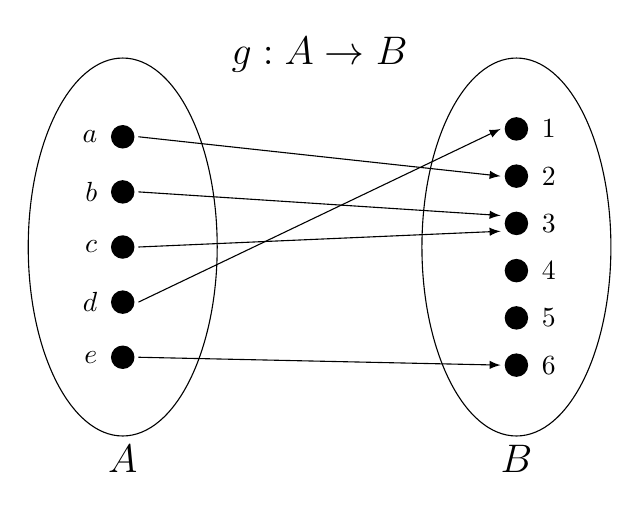
\begin{tikzpicture}[scale=1]
        \foreach \x in {1,...,6}
        {
            \node at (5, -\x*0.6)[circle,fill,inner sep=3pt]{};
            \draw[shift={(5.2, -\x*0.6)}] node[right] {$\x$};
        }
        \draw (5,-2.1) ellipse (1.2 and 2.4);

        \foreach \x/\s in  {1/a,2/b,3/c,4/d,5/e}
        {
            \node at (0, -\x*0.7)[circle,fill,inner sep=3pt]{};
            \draw[shift={(-0.2, -\x*0.7)}] node[left] {$\s$};
        }
        \draw (0,-2.1) ellipse (1.2 and 2.4);

        \draw[-latex] (0.2,-0.7) -- (4.8,-1.2); 
        \draw[-latex] (0.2,-1.4) -- (4.8,-1.7); 
        \draw[-latex] (0.2,-2.1) -- (4.8,-1.9); 
        \draw[-latex] (0.2,-2.8) -- (4.8,-0.6); 
        \draw[-latex] (0.2,-3.5) -- (4.8,-3.6);
        
        \node[below] at (0, -4.5){\Large $A$};
        \node[below] at (5, -4.5){\Large $B$};
        \node[above] at (2.5, 0){\Large $g:A \to B$};
    \end{tikzpicture}}
\end{center}

尽管如此,这种表示确实在某种程度上\emph{体现}了函数的核心思想。图中用椭圆分别标识定义域 $A$ 和值域 $B$,元素以椭圆内的标记点表示。我们根据函数 $g: A \to B$ 在点间绘制箭头。

该方法常用于探索函数特性或构造反例以驳斥某些论断。通过绘制点与箭头并尝试不同连接方式,我们能逐步构建例子的基本\emph{框架}。随后,为图中元素分配具体名称和公式,使其严谨化。

在后续讨论中,我们将用示意图辅助说明某些属性和概念,同时辅以更严格的陈述或描述。我们鼓励你也采用这一方法。

\clearpage

% !TeX root = ../../../book.tex

\subsection{习题}

\subsubsection*{温故知新}

以口头或书面的形式简要回答以下问题。这些问题全都基于你刚刚阅读的内容,如果忘记了具体定义、概念或示例,可以回顾相关内容。确保在继续学习之前能够自信地作答这些问题,这将有助于你的理解和记忆!

\begin{enumerate}[label=(\arabic*)]
    \item 在不查阅资料的情况下,写出\textbf{函数}的定义。然后,与我们的定义进行比较。你的定义是否传达了相同的信息?如果没有,遗漏了什么内容?
    \item 函数的\textbf{定义域}和\textbf{值域}有何区别?
    \item 函数\textbf{良好定义}的含义是什么?
    \item 什么是\textbf{恒等函数}?它是如何定义的?
    \item 如何证明两个函数\textbf{相等}?
\end{enumerate}

\subsubsection*{小试牛刀}

尝试解答以下问题。这些题目需动笔书写或口头阐述答案,旨在帮助你熟练运用新概念、定义及符号。题目难度适中,确保掌握它们将大有裨益!

\begin{enumerate}[label=(\arabic*)]
    \item 用符号定义函数:输入整数,输出其绝对值的平方根。\\
          该函数的定义域是什么?值域是什么?
    \item 用符号定义函数:输入一对自然数,输出其算术平均数。\\
          该函数的定义域是什么?值域是什么?
    \item 设 $A = \{-2, -1, 0, 1, 2\}$,定义 $g : A \to A$ 为 $\forall x \in A \centerdot g(x) = x^2 - 3$。绘制示意图来判断 $g$ 是否是良好定义的?
    \item 设 $X$ 为任意集合。用符号定义函数:输入 $X$ 的\emph{子集},输出其在 $X$ 上的补集。\\
          该函数的定义域是什么?值域是什么?
    \item 设 $B = \{-1, 0, 1\}$。定义 $h : B \to B$ 为 $\forall b \in B \centerdot h(b) = b^3$。这与哪个特殊函数相等?
    \item 设 $f : \mathbb{Z} \times \mathbb{Z} \to \mathbb{N}$ 为 $\forall (x, y) \in \mathbb{Z} \times \mathbb{Z} \centerdot f(x, y) = \frac{1}{2}|x + 1| \cdot |y|$。这是一个良好定义的函数吗?为什么?
\end{enumerate}

\newpage
% !TeX root = ../../../book.tex
\section{像与原像}\label{sec:section7.3}

% !TeX root = ../../../book.tex

\subsection{像:定义与示例}




% !TeX root = ../../../book.tex

\subsection{关于像的证明}

你可能已经通过研究我们之前看到的一些例子发现了以下事实。无论如何,我们都可以通过使用像的定义来陈述和证明这个命题。请注意,这是关于\emph{任意}函数的命题;无论 $f$ 是什么,它都成立!

\begin{proposition}\label{prop:proposition7.3.6}
    设 $A,B$ 为集合,$f:A \to B$ 为函数。设 $S, T \subseteq A$,则
    \[Im_f (S \cap T) \subseteq Im_f (S) \cap Im_f (T)\]
\end{proposition}

\begin{proof}
    设 $z \in Im_f (S \cap T)$ 为任意固定元素。这意味着 $\exists a \in S \cap T$ 使得 $f(a) = z$。给定这样的 $a$。

    因为 $a \in S \cap T$,所以我们知道 $a \in S$ 且 $a \in T$。

    因此,根据像的定义,$z \in Im_f (S)$ 且 $z \in Im_f (T)$。

    根据交集的定义,我们推导出 $z \in Im_f (S) \cap Im_f (T)$。

    这证明了我们要证明的集合包含关系。
\end{proof}

为什么我们没有在这里声明\emph{相等}呢?实际上,相等\emph{不一定成立}!也就是说,存在至少一个函数使得逆包含关系 --- 即 $Im_f (S) \cap Im_f (T) \subseteq Im_f (S \cap T)$ --- 不成立。我们将在下面提供这样一个函数的例子。

(你应该尝试想出一个逆包含关系\emph{成立}的函数的例子。这样,我们就能证明不能\emph{必然}得出这个包含关系成立的结论!)

我们将通过示意图来展示一个具有特定属性的例子。然后,我们会使用这个例子来正式\emph{定义}一个函数,并说明其属性,指出这些属性如何与我们的论点相一致。

需要注意的是,使用这种方法是完全可行的,只要你之后补充一个正式的定义。仅仅依靠示意图作为``证明''是不够严谨的,但它确实能帮助你更好地构思证明的\emph{思路}。

另外,在这种情况下,没有必要构造\emph{复杂}或\emph{有趣}的反例。如果你想\emph{反驳}一个全称量化陈述,只需要\emph{一个}有效的例子就可以了!特别是,不要觉得你需要定义一个通过\emph{公式}处理\emph{数字}的函数。有时,这反而会增加难度!通常,反例可以通过只包含几个(如两个或三个)元素的集合来构造。\\

\begin{example}
    我们声称存在集合 $A,B,S,T$ 和函数 $f : A \to B$,使得 $Im_f (S) \cap Im_f (T) \nsubseteq Im_f (S \cap T)$。让我们看看如何构造这样的例子。基于前面的讨论,我们将尝试构造一个包含大约三个元素的集合的例子。我们先令 $A = \{1, 2, 3\}$ 并定义 $f(1)$:

    \begin{center}
        {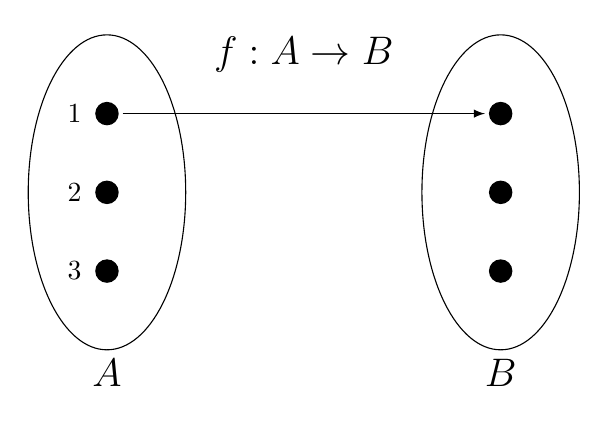
\begin{tikzpicture}[scale=1]
            \foreach \x in  {1,2,3}
            {
                \node at (5, -\x)[circle,fill,inner sep=3pt]{};
            }
            \draw[shift={(5.2, -1)}] node[right] {$\bigstar$};
            \draw (5,-2) ellipse (1 and 2);
    
            \foreach \x in  {1,2,3}
            {
                \node at (0, -\x)[circle,fill,inner sep=3pt]{};
                \draw[shift={(-0.2, -\x)}] node[left] {$\x$};
            }
            \draw (0,-2) ellipse (1 and 2);
    
            \draw[-latex] (0.2,-1) -- (4.8,-1); 
            
            \node[below] at (0, -4){\Large $A$};
            \node[below] at (5, -4){\Large $B$};
            \node[above] at (2.5, -0.6){\Large $f:A \to B$};
        \end{tikzpicture}}
    \end{center}

    为了便于定义,我们令 $S = \{1, 2\}$。让 $S$ 中包含两个元素似乎更合理,因此我们做出这个选择。此外,我们应该设 $f(1) \ne f(2)$,否则 $Im_f(S)$ 只会包含一个元素,这样 $S$ 有两个元素就没有意义了。因此,我们定义 $f(2)$:

    \begin{center}
        {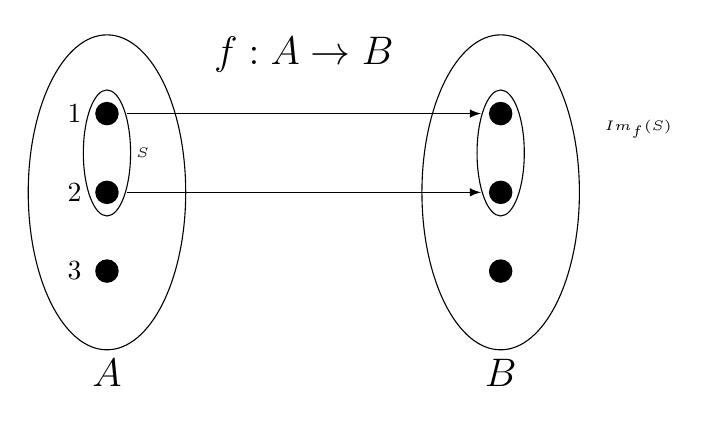
\begin{tikzpicture}[scale=1]
            \foreach \x in  {1,2,3}
            {
                \node at (5, -\x)[circle,fill,inner sep=3pt]{};
            }
            \draw[shift={(5.2, -1)}] node[right] {$\bigstar$};
            \draw[shift={(5.2, -2)}] node[right] {$\square$};
            \draw (5,-2) ellipse (1 and 2);
            \draw (5,-1.5) ellipse (0.3 and 0.8);
    
            \foreach \x in  {1,2,3}
            {
                \node at (0, -\x)[circle,fill,inner sep=3pt]{};
                \draw[shift={(-0.2, -\x)}] node[left] {$\x$};
            }
            \draw (0,-2) ellipse (1 and 2);
            \draw (0,-1.5) ellipse (0.3 and 0.8);
    
            \draw[-latex] (0.25,-1) -- (4.75,-1);
            \draw[-latex] (0.25,-2) -- (4.75,-2); 
    
            \node[right] at (0.25, -1.5){\tiny $S$};
            \node[right] at (6.2, -1.2){\tiny $Im_f(S)$};
            \node[below] at (0, -4){\Large $A$};
            \node[below] at (5, -4){\Large $B$};
            \node[above] at (2.5, -0.6){\Large $f:A \to B$};
        \end{tikzpicture}}
    \end{center}

    现在,我们需要选择集合 $T$。如果让 $S$ 和 $T$ 互不相交 ($S \cap T = \varnothing$) 会很有趣,而如果让 $T$ 包含 $S$ ($T \supseteq S$),处理起来可能会很复杂。因此,我们设 $T = \{2, 3\}$。接下来,我们只需要定义 $f(3)$。在考虑每种情况时,请参照上面的示意图,想象画一个箭头来表示 $f(3)$。

    \begin{itemize}
        \item 如果 $f(3) = f(2) = \square$。\\
            这种情况下,$Im_f(T) = \{\square\}$,所以 $Im_f (S) \cap Im_f (T) = \{\square\}$。而 $Im_f (S \cap T) = \{\square\}$, 这行不通。
        \item 如果 $f(3)$ 等于其他值,比如 $\smiley{}$。\\
            这也行不通。我们会得到 $Im_f (S) \cap Im_f (T) = \{\square\} = Im_f (S \cap T)$。
        \item 如果 $f(3) = f(1) = \bigstar$。\\
            这似乎可以!
    \end{itemize}

    \begin{center}
        {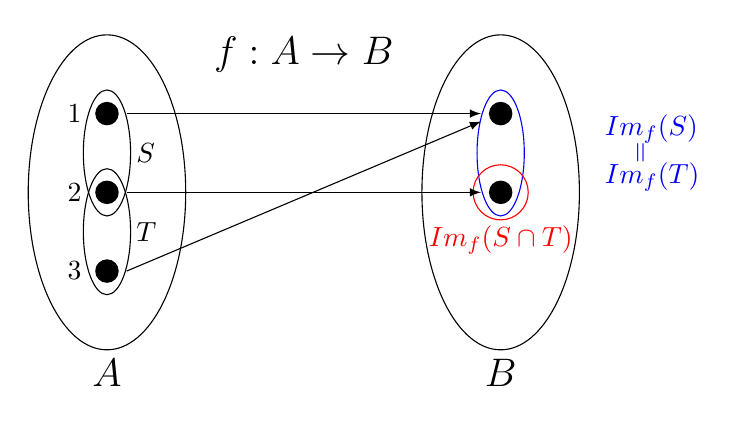
\begin{tikzpicture}[scale=1]
            \foreach \x in {1,2}
            {
                \node at (5, -\x)[circle,fill,inner sep=3pt]{};
            }
            \draw[shift={(5.2, -1)}] node[right] {$\bigstar$};
            \draw[shift={(5.2, -2)}] node[right] {$\square$};
            \draw (5,-2) ellipse (1 and 2);
            \draw[blue] (5,-1.5) ellipse (0.3 and 0.8);
            \draw[red] (5,-2) circle (0.35);
            \node[below, red] at (5, -2.3){$Im_f(S \cap T)$};
    
            \foreach \x in  {1,2,3}
            {
                \node at (0, -\x)[circle,fill,inner sep=3pt]{};
                \draw[shift={(-0.2, -\x)}] node[left] {$\x$};
            }
            \draw (0,-2) ellipse (1 and 2);
            \draw (0,-1.5) ellipse (0.3 and 0.8);
            \draw (0,-2.5) ellipse (0.3 and 0.8);
    
            \draw[-latex] (0.25,-1) -- (4.75,-1);
            \draw[-latex] (0.25,-2) -- (4.75,-2); 
            \draw[-latex] (0.25,-3) -- (4.75,-1.1); 
    
            \node[right] at (0.25, -1.5){$S$};
            \node[right] at (0.25, -2.5){$T$};
            \node[right, blue] at (6.2, -1.2){$Im_f(S)$};
            \node[right, blue, anchor=center, rotate=90] at (6.8, -1.5){$=$};
            \node[right, blue] at (6.2, -1.8){$Im_f(T)$};
            \node[below] at (0, -4){\Large$A$};
            \node[below] at (5, -4){\Large$B$};
            \node[above] at (2.5, -0.6){\Large $f:A \to B$};
        \end{tikzpicture}}
    \end{center}
\end{example}

我们已经成功实现 $Im_f (S) \cap Im_f (T)$ 是 $Im_f (S \cap T)$ 的\emph{真}超集。

回顾一下我们的构造过程,看看你是否理解我们的思路。我们需要遵守哪些限制?在哪些方面有选择的自由?我们最终决定怎么做?

需要说明的是,这绝对不是\emph{唯一的}例子!你也可以尝试想出其他的例子!

现在,我们只需要用我们构造的最终示意图来定义一个例子,并证明它的有效性。我们开始吧!

\begin{proof}
    定义 $A = \{1, 2, 3\}, B = \{\bigstar, \square\}$。

    定义 $f : A \to B$ 为 $f(1) = \bigstar, f(2) = \square, f(3) = \bigstar$。

    定义 $S = \{1, 2\}, T = \{2, 3\}$。

    易得 $S \cap T = \{2\}$,所以 $Im_f (S \cap T) = \{f(2)\} = \{\square\}$。

    然而,$Im_f (S) = Imf (T) = B$,所以 $Im_f (S) \cap Im_f (T) = \{\bigstar, \square\} \ne \{\square\}$。

    因为 $\bigstar \in Im_f (S) \cap Im_f (T)$ 而 $\bigstar \notin Im_f (S \cap T)$,这证明了我们的声明。
\end{proof}

我们已经展示了如何\textbf{证明}关于任意函数和像的声明,以及如何通过\textbf{构造}具体反例来\textbf{反驳}一个声明。在下面的练习中,你将会遇到类似的问题。有时,你需要判断一个声明是否为真。(在这里,我们已经提前告诉你哪个声明是正确的。)我们建议你可以尝试以下两种方法:
\begin{enumerate}[label=(\arabic*)]
    \item 试着证明这个声明,看看是否在某个地方会出现问题;
    \item 试着构造一个反例,看看是否会遇到困难。
\end{enumerate}
如果你完成了上面任意一项……太好了,你已经解决了这个问题!但如果你感到困难,这可能会帮助你更好地理解问题的本质。

具体来说,我们要求你用 ``$\cup$'' 代替 ``$\cap$'' 来重新审视我们上面讨论的命题。你认为会有什么不同吗?试试看吧!

% !TeX root = ../../../book.tex

\subsection{原像:定义与示例}


% !TeX root = ../../../book.tex

\subsection{关于原像的证明}

请注意,以下命题是\textbf{相等}关系。将其与命题 \ref{prop:proposition7.3.6} 进行比较,后者是一个关于\emph{像}的类似陈述,但它只是集合包含关系。很有意思,对吧?

\begin{proposition}
    设 $A,B$ 为集合,$f:A \to B$ 为函数。设 $X, Y \subseteq B$,则
    \[PreIm_f (X \cap Y) = PreIm_f (X) \cap PreIm_f (Y)\]
\end{proposition}

注意下面的证明是如何直接运用原像的形式定义的。我们将直接开始证明这两部分。练习部分将要求你用 ``$cup$'' 替换 ``$cap$'' 来验证这个论断。

\begin{proof}
    设 $x \in PreIm_f (X \cap Y)$ 为任意固定元素。

    根据原像的定义,这意味着 $f(x) \in X \cap Y$,即 $f(x) \in X$ 且 $f(x) \in Y$。

    因为 $f(x) \in X$,根据原像的定义,这意味着 $x \in PreIm_f (X)$。同理,因为 $f(x) \in Y$,这意味着 $x \in PreIm_f (Y)$。

    根据交集的定义,我们推导出 $x \in PreIm_f(X) \cap PreIm_f(Y)$。

    这证明了 $PreIm_f(X \cap Y) \subseteq PreIm_f(X) \cap PreIm_f(Y)$。\\

    接着,设 $y \in PreIm_f(X) \cap PreIm_f(Y)$ 为任意固定元素。

    根据交集的定义,这意味着 $y \in PreIm_f (X)$ 且 $y \in PreIm_f (Y)$。

    因为 $y \in PreIm_f (X)$,根据原像的定义,我们可以推导出 $f(y) \in X$。同理,因为 $y \in PreIm_f (Y)$,我们可以推导出 $f(y) \in Y$。

    根据交集的定义,这告诉我们 $f(y) \in X \cap Y$。

    根据原像的定义,可得 $y \in PreIm_f(X \cap Y)$。

    这证明了 $ PreIm_f(X \cap Y) \supseteq PreIm_f(X) \cap PreIm_f(Y)$。 \\

    综上,利用双重包含论证,我们证明了该命题。
\end{proof}

读到这里你可能会想,``这种证明方法是怎么想出来的?''其实,这样的结果并没有什么特别的巧思。我们只是直接引用定义,然后一切就变得顺理成章了。如果你在解决问题时感到困惑,或者不知道从哪里开始……那就写下相关的定义,试着把它们应用到你要证明的陈述上,看看会有什么结果!

\subsubsection*{像和原像的证明}

让我们来看一个涉及本节中两个概念的例子。我们将证明一个包含关系,并在练习中要求你证明另一个包含关系不成立。

\begin{proposition}\label{prop:proposition7.3.12}
    设 $A,B$ 为集合,$f:A \to B$ 为函数。设 $Y \subseteq B$,则
    \[Im_f \big(PreIm_f (Y)\big) \subseteq Y\]
\end{proposition}

\begin{proof}
    设 $b \in Im_f \big(PreIm_f (Y)\big)$ 为任意固定元素。

    根据像的定义,这意味着 $\exists a \in PreIm_f (Y) \centerdot f(a) = b$。给定这样的 $a$。

    因为 $a \in PreIm_f (Y)$,根据原像的定义,这意味着 $f(a) \in Y$。

    因为 $b = f(a)$ 且 $f(a) \in Y$,这意味着 $b \in Y$。

    这就证明了该命题。
\end{proof}


% !TeX root = ../../../book.tex

\subsection{习题}

\subsubsection*{温故知新}

以口头或书面的形式简要回答以下问题。这些问题全都基于你刚刚阅读的内容,所以如果忘记了具体的定义、概念或示例,可以回去重读相关部分。确保在继续学习之前能够自信地回答这些问题,这将有助于你的理解和记忆!

\begin{enumerate}[label=(\arabic*)]
    \item \textbf{像}与\textbf{原像}之间有什么区别?
    \item 假设 $f : A \to B$ 是一个函数。$PreIm_f (B)$ 表示什么?
    \item 假设 $g : \mathbb{R} \to \mathbb{R}$ 是一个函数。为什么表达式 $Im_g(0)$ 不是一个正确的陈述?你认为写出该表达式的人是什么意思?
    \item 假设 $f : A \to B$ 是一个函数且 $Y \subseteq B$。如果 $PreIm_f (Y) = \varnothing$,这意味着什么?这有可能吗?
    \item 假设 $f : A \to B$ 是一个函数且 $X \subseteq A$。如果 $Im_f (X) = \varnothing$,这意味着什么?这有可能吗?
\end{enumerate}

\subsubsection*{小试牛刀}

尝试回答以下问题。这些题目要求你实际动笔写下答案,或(对朋友/同学)口头陈述答案。目的是帮助你练习使用新的概念、定义和符号。题目都比较简单,确保能够解决这些问题将对你大有帮助!

\begin{enumerate}[label=(\arabic*)]
    \item 设函数 $h : \mathbb{R} - \{-1\} \to \mathbb{R}$ 定义为 $\forall x \in \mathbb{R} - \{-1\} \centerdot h(x) = \frac{x}{1+x}$。\\
        证明 $Im_h(\mathbb{R} - \{-1\}) = \mathbb{R} - \{-1\}$。\\
        然后,定义 $P = \{y \in \mathbb{R} \mid y > 1\}, U = \{y \in \mathbb{R} \mid y > -1\}$。 \\
        证明 $PreIm_h(P) = U$。
    \item 设 $f:A \to B$ 为函数。设 $S,T \subseteq A$。对于下列声明,\textbf{证明}他们成立,或找出\textbf{反例}。
        \begin{enumerate}[label=(\alph*)]
            \item $Im_f (S \cup T) \subseteq Im_f (S) \cup Im_f (T)$
            \item $Im_f (S \cup T) \supseteq Im_f (S) \cup Im_f (T)$
        \end{enumerate}
    \item 设 $f:A \to B$ 为函数。设 $Y,Z \subseteq B$。对于下列声明,\textbf{证明}他们成立,或找出\textbf{反例}。
        \begin{enumerate}[label=(\alph*)]
            \item $PreIm_f (Y \cup Z) \subseteq PreIm_f (Y) \cup PreIm_f (Z)$
            \item $PreIm_f (Y \cup Z) \supseteq PreIm_f (Y) \cup PreIm_f (Z)$
        \end{enumerate}
    \item 回看命题 \ref{prop:proposition7.3.12},考虑\emph{反方向}包含关系
        \[Im_f \big(PreIm_f (Y)\big) \supseteq Y\]
        通过构造一个具体的反例并证明其有效性,来\textbf{反驳}以下声明:对于任意函数 $f : A \to B$ 和任意 $Y \subseteq B$,该声明都成立。
\end{enumerate}

\newpage
% !TeX root = ../../../book.tex

\section{函数的性质}\label{sec:section7.3.5}

% !TeX root = ../../../book.tex

\subsection{满射函数}

你可能会问……如果我们能确定给定函数定义域的像,为什么还要用比这个像更大的值域呢?例如,函数 $f : \mathbb{R} \to \mathbb{R}$ 定义为 $f(x) = x^2$ 是良好定义的函数,但如果把值域改为非负实数集也不会有任何影响。这样做甚至更好,因为函数不会``遗漏''任何值域中的元素!如果你有这样的想法,那么你已经理解了我们接下来的定义,这个定义准确地概括了函数的这一特性:值域和定义域的像是同一个集合这种情况。

\subsubsection*{定义}

\begin{definition}
    设 $A,B$ 为集合,$f:A \to B$ 为函数。我们说 $f$ 是\dotuline{满射}函数,当且仅当 $Im_f (A) = B$。

    同样地,我们可以说 ``$f$ 是满射的''(形容词形式),或者说 ``$f$ 是一个满射''(名词形式)。

    回到像的定义,我们可以用一个量化陈述来等价地描述这个性质:
    \[f \;\text{是满射} \iff \forall b \in B \centerdot \exists a \in A \centerdot f(a) = b\]
    也就是说,$f$ 是满射当且仅当每个输出至少有一个对应的输入。
\end{definition}

想一想为什么这个定义的第二种形式实际上与第一种形式是相同的。性质 $Im_f (A) = B$ 是关于集合的陈述。根据定义,我们已经知道 $Imf (A) \subseteq B$(像中的任何元素都不能``超出''值域),所以这个进一步的性质意味着 $B \subseteq Im_f (A)$。这正是定义的第二种形式所说的:值域的每个元素都满足像元素的定义。

另外,注意定义中没有说我们找到的与 $b$ 对应的 $a$ 必须是唯一的!这个性质所要求的只是,对于每个 $b \in B$,我们可以找到\emph{至少一个} $a \in A$ 满足 $f(a) = b$。可能有多个,也可能只有一个。这无关紧要,只要不是\emph{一个都没有}就行。

在示意图中,\emph{满射}的性质意味着什么?由于值域的每个元素都被函数``命中'',这意味着示意图右侧的每个点都有一个箭头指向它。(记住:这种启发式语言是可以记住的 --- 毕竟我们用它来帮助描述这些概念 --- 但这不构成证明。在你用于证明的任何语句中,应该使用着更严格的陈述,使用数学语言和/或逻辑符号。)为什么我们会关心这样的性质?一般来说,声明一个函数的像究竟是什么可能很困难,我们可能(首先)只能声明值域是什么。实际上证明值域的所有元素都是函数的输出可以提供额外的、有用的信息!

\subsubsection*{满射定义的否定}

通常,我们会先定义一个函数,然后问:这是一个满射吗?如果我们认为一个函数是满射,我们应该通过证明值域和像是同一集合来证实。如果我们认为它不是满射,我们应该通过找到一个反例来证明它不是满射。让我们来看一下满射函数定义的逻辑否定:
\[\neg (\forall b \in B \centerdot \exists a \in A \centerdot f(a) = b) \iff \exists b \in B \centerdot \forall a \in A \centerdot f(a) \ne b\]
也就是说,要证明函数 $f$ 不是满射,我们必须找到一个不在像中的值域元素。这需要一些验算和直觉来识别这样的元素 $b$。接下来,我们必须以某种方式证明没有任何 $a$ 满足 $f(a) = b$。我们可以通过取任意 $a \in A$ 并解释为什么 $f(a) \ne b$ 来直接证明这一点。或者,我们可以通过反证法来证明:假设存在一个 $a \in A$ 使得 $f(a) = b$,然后找出矛盾。这两种方法都是合理的,并且是逻辑等价的。

\subsubsection*{示例}

让我们通过几个例子来看看这些技术是如何应用的。对于其中一些例子,我们可以借助图形直觉或尝试一些测试案例来进行\emph{猜想},但最终我们需要通过\emph{证明}某些逻辑陈述来验证我们的观点。\\

\begin{example}
    考虑函数 $p : \mathbb{N} \times \mathbb{N} \to \mathbb{N}$ 定义为 $p(a,b) = ab$。$p$ 是满射吗?

    答案是肯定的。我们可以设 $a$ 为 $1$,则函数的输出就是 $b$。让我们通过证明来让这个观察更加正式:

    \begin{proof}
        设 $n \in \mathbb{N}$ 为任意固定自然数。定义 $(a, b) = (1, n)$。

        不难发现 $(1, n) \in \mathbb{N} \times \mathbb{N}$ 且 $p(1, n) = 1 \cdot n = n$。

        因为 $n$ 是任意的,这证明了 $p$ 是满射。
    \end{proof}
\end{example}

\begin{example}
    设 $C$ 为美国所有汽车的集合。设 $S$ 为所有由字母和数字组成的长度最多为 $7$ 的字符串的集合(这些是可能出现在汽车牌照上的\emph{潜在}字符串)。

    设 $f : C \to S$ 定义为输入一辆车,输出其牌照字符串。函数 $f$ 是满射吗?

    不,绝对不是!也许你没注意到,\emph{敏感词}是不允许出现在牌照上的!所以,肯定存在许多在美国牌照上绝对不会出现的字符串。(我们就不列举了,你可以自己想一些例子……)

    因为我们展示了 $S$ 中至少有一个元素\emph{不是} $Im_f (C)$ 的元素,因此我们已经证明了 $f$ 不是一个满射。
\end{example}

\begin{example}
    设函数 $d : \mathbb{N} \times \mathbb{N} \to \mathbb{Z}$ 定义为
    \[\forall (a, b) \in \mathbb{N} \times \mathbb{N} \centerdot d(a, b) = a - b\]
    我们来判断 $d$ 是否是满射,并证明我们的结论。

    我们可以先尝试一些``较小的''输入值。在下表中,左列表示 $a$,顶行表示 $b$,表格中的值是 $d(a, b) = a - b$:
    \begin{center}
        \begin{tabular}{c|ccccc}
              & 1 & 2  & 3  & 4  & 5  \\
            \hline
            1 & 0 & -1 & -2 & -3 & -4 \\
            2 & 1 & 0  & -1 & -2 & -3 \\
            3 & 2 & 1  & 0  & -1 & -2 \\
            4 & 3 & 2  & 1  & 0  & -1 \\
            5 & 4 & 3  & 2  & 1  & 0  \\
        \end{tabular}
    \end{center}
    看起来所有的整数 $z \in \mathbb{Z}$ 都会出现在这个表格中。然而,它们不会全部出现在某一特定的行或列中。相反,所有非负整数似乎都出现在第一列,而所有非正整数似乎都出现在第一行。让我们根据这些观察来写一个证明。我们将取任意整数 $z \in \mathbb{Z}$,并分两种情况讨论:如果 $z \ge 0$,我们将采取一种方法;如果 $z < 0$,我们将采取另一种方法。只要我们在这两种情况下都成功,我们就证明了 $d$ 是一个满射。

    \begin{proof}
        我们声称 $d$ 是满射。

        设 $z \in \mathbb{Z}$ 是任意固定整数。我们要证明 $\exists (a, b) \in \mathbb{N} \times \mathbb{N} \centerdot d(a, b) = z$。为此,考虑如下两种情况:
        \begin{enumerate}[label=(\arabic*)]
            \item 假设 $z \ge 0$,则定义 $(a, b) = (z + 1, 1)$。\\
                  因为 $z \ge 0$,我们知道 $z+1 \ge 1$,因此 $z+1 \in \mathbb{N}$。这确保了 $(z + 1, 1) \in \mathbb{N} \times \mathbb{N}$。\\
                  此时 $d(z + 1, 1) = (z + 1) - 1 = z$。
            \item 假设 $z < 0$,则定义 $ (a, b) = (1, -z + 1)$。\\
                  因为 $z < 0$,我们知道 $-z > 0$,因此 $-z+1 > 1$,这意味着 $-z+1 \in \mathbb{N}$。这确保了 $(1, -z+1) \in \mathbb{N} \times \mathbb{N}$。\\
                  此时 $d(1, -z + 1) = 1 - (-z + 1) = z$。
        \end{enumerate}
        无论哪种情况,我们都可以定义 $(a, b) \in \mathbb{N} \times \mathbb{N} \centerdot d(a, b) = z$。因为 $z \in \mathbb{Z}$ 是任意整数,所以这证明了 $d$ 是一个满射。
    \end{proof}
\end{example}

\begin{example}
    设函数 $g : \mathbb{R} - \{-1\} \to \mathbb{R}$ 定义为
    \[\forall x \in \mathbb{R} - \{-1\} \centerdot g(x) = \frac{x}{1+x}\]
    (注意,我们为什么从定义域中移除了 $-1$。这是为了确保 $g$ 是\emph{良好定义的}。)

    我们来判断 $g$ 是否是满射,并证明我们的结论。如前所述,我们可以通过做一些验算来确定这一点:我们可以尝试代入一些 $x$ 的值,让 $x$ 非常接近 $-1$ 或变得越来越大,以测试``极端情况''……这些都有助于我们绘制函数图像,或者我们可以使用绘图软件直接画出函数图像:

    \begin{center}
        \begin{tikzpicture}
            \begin{axis}[
                    ymin=-1.5,
                    ymax=3.5,
                    xmin=-5,
                    xmax=5,
                    minor tick num=3,
                    axis lines*=middle,
                    xtick align=inside,
                    ytick align=inside
                ]
                \addplot[blue, line width=1pt, domain=-5:-1.1, samples=40, smooth] {x/(1+x)};
                \addplot[blue, line width=1pt, domain=-0.9: 5, samples=60, smooth] {x/(1+x)};
                \addplot[black, dashed, domain=-5:5, samples=2] {1};
            \end{axis}
        \end{tikzpicture}
    \end{center}

    然而,无论是哪种绘图方式,都不能构成\emph{证明}!它只是帮助我们观察到函数 $g$ \emph{不是}满射。在 $y = 1$ 处似乎有一个水平渐近线。也就是说,函数 $g$ 只会无限接近 $1$,但永远无法``达到'' $1$,。根据我们对\emph{满射}的定义,$g$ 显然不是满射!

    现在尝试证明这一点。你如何证明元素 $-1 \in \mathbb{R}$ \emph{不是}像 $Im_g(\mathbb{R})$ 的元素呢?试试看吧!然后继续阅读我们的证明。

    我们将给出\emph{两个}证明供你比较和对比。它们都证明了同一个结论 --- $g$ 不是满射。其中一个采用反证法,另一个采用直接证法(通过分情况讨论)。你觉得哪个更好?你是否也想到了其中一种证法?哪个更容易理解?对于这些问题,我们没有明确的观点;这两个证明都是有效的!

    \begin{proofs}{证明 1 (直接证法)}
        设 $x \in \mathbb{R} - \{-1\}$ 为任意固定元素。我们要证明 $g(x) \ne 1$。考虑如下两种情况:
        \begin{itemize}
            \item 假设 $x > -1$。\\
                  这意味着 $x+1>0$,所以 $\frac{1}{x+1}>0$。我们还知道 $x+1>x$ 对于所有 $x \in \mathbb{R}$ 都成立。不等式两边同时乘以一个正项 $\frac{1}{x+1}$ 得 $1 > \frac{x}(x+1)$,即 $g(x) = \frac{x}(x+1) \ne 1$。
            \item 假设 $x < -1$。\\
                  这意味着 $x+1<0$,所以 $\frac{1}{x+1}<0$。我们还知道 $x+1>x$ 对于所有 $x \in \mathbb{R}$ 都成立。不等式两边同时乘以一个负项 $\frac{1}{x+1}$ 得 $1 < \frac{x}(x+1)$,即 $g(x) =  \frac{x}(x+1) \ne 1$。
        \end{itemize}
        无论哪种情况都有 $g(x) \ne 1$。因为上述两种情况覆盖了所有可能的情况,并且 $x \in \mathbb{R} - \{-1\}$ 是任意的,这证明了
        \[1 \notin Im_g(\mathbb{R} - \{-1\})\]
        所以 $g$ 不是满射。
    \end{proofs}

    请注意,证明 1 揭示了图像的一个有趣现象:该函数在 $x = -1$ 的左侧图像位于水平渐近线之上,而在 $x = -1$ 的右侧图像位于渐近线之下。

    \begin{proofs}{证明 2 (反证法)}
        为了引出矛盾而假设 $g$ 是满射。这意味着
        \[\forall y \in \mathbb{R} \centerdot y \in Im_g(\mathbb{R} - \{-1\})\]
        特别地,我们知道 $1 \in Im_g(\mathbb{R} - \{-1\})$,所以 $\exists x \in \mathbb{R} - \{-1\} \centerdot g(x) = 1$。给定这样的 $x$。

        这意味着 $g(x) = \frac{x}{x+1} = 1$。两边同时乘以分母得 $x = x + 1$。两边同时减去 $x$ 得 $0 = 1$,显然这是一个矛盾。$
            \hashx$

        因此,$1 \notin Im_g(\mathbb{R} - \{-1\})$,所以 $g$ 不是满射。
    \end{proofs}

    请注意,证明 2 虽然确实证明了 $g$ 不是满射,但没有提供其他关于函数行为的信息(不像证明 1 那样)。

    接下来,我们来讨论一个与函数密切相关的性质。
\end{example}

% !TeX root = ../../../book.tex

\subsection{关于像的证明}


% !TeX root = ../../../book.tex

\subsection{映射的证明技巧}

为了总结本节内容,我们提供以下\textbf{证明模板},用于证明或证伪函数是否为单射 (Injection) 或满射 (Surjection)。我们通常用术语``映射 (Jection)''统称这两种属性。

\subsubsection*{证明函数 $f$ 是满射}

\begin{enumerate}
    \item 设 $b \in B$ 为任意固定元素。
    \item 定义 $a = \underline{\qquad\qquad}$。
    \item 证明 $a \in A$。
    \item 证明 $f(a) = b$。
    \item 这证明了 $b \in \im_f(A)$。因此,$\im_f(A)=B$,故 $f$ 是满射。
\end{enumerate}

\subsubsection*{证明函数 $f$ 不是满射}

\begin{enumerate}
    \item 定义 $b = \underline{\qquad\qquad}$。
    \item 证明 $b \in B$。
    \item 设 $a \in A$ 为任意固定元素。
    \item 证明 $f(a) \ne b$。\\
        (或者,假设 $f(a) = b$,推导出矛盾。)
    \item 这证明了 $\exists b \in B \centerdot b \notin \im_f(A)$。故 $f$ 不是满射。
\end{enumerate}

\subsubsection*{证明函数 $f$ 是单射}

\begin{enumerate}
    \item 设 $x,y \in A$ 为任意固定元素。
    \item 假设 $f(x) = f(y)$。
    \item 推导出 $x = y$。
\end{enumerate}

或者

\begin{enumerate}
    \item 设 $x,y \in A$ 为任意固定元素。
    \item 假设 $x \ne y$。
    \item 推导出 $f(x) \ne f(y)$。
\end{enumerate}

\subsubsection*{证明函数 $f$ 不是单射}

\begin{enumerate}
    \item 定义 $x = \underline{\qquad\qquad}$,定义 $y = \underline{\qquad\qquad}$。
    \item 证明 $x \in A, y \in B$。
    \item 证明 $x \ne y$。
    \item 证明 $f(x) = f(y)$。
\end{enumerate}

\subsubsection*{证明函数 $f$ 是双射}

\begin{enumerate}
    \item 证明 $f$ 为单射。
    \item 证明 $f$ 为满射。
\end{enumerate}

% !TeX root = ../../../book.tex

\subsection{双射}

你可能已经猜到本节要讨论的内容。回顾我们刚刚研究的两个核心函数性质:\emph{满射性 (Surjectivity)} 和\emph{单射性 (Injectivity)}。若函数同时具备这两个性质会如何?这意味着值域中每个元素在定义域中\emph{至少}有一个对应元素(满射性),且\emph{至多}有一个对应元素(单射性)。换言之,每个输出都有且仅有一个输入与之对应!这一关键性质将成为讨论\emph{基数}(集合大小)的基础。让我们先给出定义,再通过示例阐明。

\subsubsection*{定义}

\begin{definition}
    设 $A, B$ 为集合,$f: A \to B$ 为函数。称 $f$ 是\dotuline{双射}函数,当且仅当 $f$ 既是单射又是满射。

    亦可表述为``$f$ 是双射的 (Bijective)''或``$f$ 为双射 (Bijection)''。

    有时我们会说``$f$ 是集合 $A$ 和 $B$ 之间的双射'',而非``从 $A$ 到 $B$'' 的双射。(下一节将解释其中原因!)
\end{definition}

从逻辑上讲,该定义是\verb|逻辑与|陈述。目前证明函数双射性的唯一方法是分别验证其满射性与单射性。反之,要证明函数非双射,只需证明其非满射或非单射(即便二者皆不成立,仅需证明其一足矣)。这里不再重复前文已经详细讨论的证明技术,我们直接考察已有案例是否为双射。\\

\begin{example}
    \begin{enumerate}[label=(\alph*)]
        \item 设函数 $p:\mathbb{N} \times \mathbb{N} \to \mathbb{N}$ 定义为 $p(a, b) = ab$ \\
            我们已经证明 $p$ 是满射但不是单射,因此它\textbf{不是}双射。
        \item 设函数 $d:\mathbb{N} \times \mathbb{N} \to \mathbb{Z}$ 定义为 $d(a, b) = a-b$ \\
            我们已经证明 $d$ 是满射但不是单射,因此它\textbf{不是}双射。
        \item 设函数 $g : \mathbb{R} - \{-1\} \to \mathbb{R}$ 定义为 
             \[\forall x \in \mathbb{R} - \{-1\} \centerdot g(x) = \frac{x}{1+x}\]
             我们已经证明 $g$ 不是满射。(具体而言,我们证明了 $ 1 \notin \im_g(\mathbb{R} - \{-1\})$。)本节的练习中,我们将要求你证明 $g$ 是单射。无论如何,$g$ 不是双射。

             然而,考虑用相同``规则''定义的函数 $h : \mathbb{R} - \{-1\} \to \mathbb{R}- \{1\}$,即
             \[\forall x \in \mathbb{R} - \{-1\} \centerdot h(x) = \frac{x}{1+x}\]
             在 \ref{sec:section7.3.5} 节的练习中,我们将要求你证明函数 $h$ 满足 $\im_h(\mathbb{R} - \{-1\}) = \mathbb{R}- \{1\}$。这证明了 $h$ 是满射。

             此外,在本节的练习中,我们还会要求你证明,通过上面这种方式定义的函数 —— 取一个单射函数,应用相同的``规则'',将值域重新定义为像集 —— 最终能够生成一个双射函数。

             综上,上述内容证明了 $h$ 是 $\mathbb{R} - \{-1\}$ 和 $\mathbb{R}- \{1\}$ 之间的\textbf{双射}。
    \end{enumerate}
\end{example}

\begin{example}
    让我们来看一个新例子。之所以选择这个例子是为了预览一些即将出现的核心思想。定义 $E \subseteq \mathbb{N}$ 为所有\emph{偶数}的集合,即:
    \[E = \{e \in \mathbb{N} \mid \exists k \in \mathbb{N} \centerdot e = 2k\}\]
    定义函数 $d : \mathbb{N} \to E$ 为 $d(n) = 2n$。我们断言 $d$ 为双射。

    \begin{proof}
        首先,证明 $d$ 是满射。
        
        给定 $e \in E$。根据 $E$ 的定义,$\exists k \in \mathbb{N}$ 使得 $e = 2k$。给定这样的 $k$。

        此时 $d(k) = 2k = e$。因为 $e$ 是任意的。故可得 $d$ 是满射。\\

        接着,证明 $d$ 是单射。

        设 $m,n \in \mathbb{N}$ 且 $d(m) = d(n)$。

        这意味着 $2m=2n$。等式两边同时除以 $2$ 得 $m=n$。因此 $d$ 是单射。\\

        综上,这证明了 $d$ 为双射。
    \end{proof}
\end{example}

我们将通过提出若干问题来激发思考:你是否觉得 $\mathbb{N}$ 和 $E$ 之间存在\emph{双射}关系有点奇怪,毕竟 $E$ 是 $\mathbb{N}$ 的\emph{真}子集?是否总能在一个集合和它的真子集之间建立双射关系?我们之前是否见过类似的例子?

\subsubsection*{启下} 

双射 $f : A \to B$ 的核心思想是将 $A$ 和 $B$ 的元素\textbf{一一对应}。这源于满射和单射的定义:每个输出都\emph{有且只有}一个输入与之对应。回顾这些性质的证明过程:当证明 $f$ 是满射时,我们表明对于值域中的每个元素,都存在至少一个定义域中的元素映射到它;当证明 $f$ 是单射时,我们表明这样的元素是唯一的。实际上,这揭示了如何``反转''函数 $f$ 的作用,从而定义一个从 $B$ 到 $A$ 的新函数。这正是我们所说的\emph{反函数}。为了严格定义这种``从值域返回到定义域''的映射,我们需要给出反函数的精确定义,并将其与双射关联起来。这些内容将在下一节详细展开。


% !TeX root = ../../../book.tex

\subsection{习题}

\subsubsection*{温故知新}

以口头或书面的形式简要回答以下问题。这些问题全都基于你刚刚阅读的内容,所以如果忘记了具体的定义、概念或示例,可以回去重读相关部分。确保在继续学习之前能够自信地回答这些问题,这将有助于你的理解和记忆!

\begin{enumerate}[label=(\arabic*)]
    \item 用\textbf{像}来定义\textbf{满射}。然后,再用量词来定义满射。
    \item 描述证明函数是\textbf{单射}的两种不同方法。
    \item 一个函数可以既是单射又是满射吗?如果可以,举一个例子。
    \item 一个函数可以既不是单射也不是满射吗?如果可以,举一个例子。
    \item 对于以下每一个示意图,判断它们是否是函数;如果是,判断它是否是单射或满射。
\end{enumerate}

\subsubsection*{小试牛刀}

尝试回答以下问题。这些题目要求你实际动笔写下答案,或(对朋友/同学)口头陈述答案。目的是帮助你练习使用新的概念、定义和符号。题目都比较简单,确保能够解决这些问题将对你大有帮助!

\begin{enumerate}[label=(\arabic*)]
    \item 假设 $f : \mathbb{R} \to \mathbb{R}$ 是\emph{单调递增}函数,即
        \[\forall x, y \in \mathbb{R} \centerdot x < y \implies f(x) < f(y)\]
        证明 $f$ 必为\emph{单射}。\\
        然后,通过定义一个递增但不是满射的函数,证明 $f$ \emph{不一定}是满射。
    \item 设函数 $g : \mathbb{R} - \{-1\} \to \mathbb{R}$ 定义为 
        \[\forall x \in \mathbb{R} - \{-1\} \centerdot g(x) = \frac{x}{1+x}\]
        $g$ 是\emph{单射}吗?请证明你的声明。
    \item 给出函数 $f : \mathcal{P}(\mathbb{N}) \to \mathbb{N}$ 为满射的一个例子,并\emph{证明}它确实是满射。\\
        (\textbf{提示}:尤其要注意 $\varnothing \in \mathcal{P}(\mathbb{N})$。你可以回看 \ref{sec:section5.5.2} 获得一些灵感……)
    \item 给出函数 $F : \mathbb{N} \to \mathcal{P}(\mathbb{N})$ 为单射的一个例子,并\emph{证明}它确实是单射。\\
        然后\emph{证明}函数 $F$ \emph{不是}满射。\\
        (注意:我们要求你\emph{在不知道函数定义的情况下},证明它不是满射。我们知道这是正确的!你将在本章后面了解到我们使用的这个小技巧……)
    \item 假设函数 $f : A \to B$ 和 $g : B \to C$ 都是满射。证明 $g \circ f:A \to C$ 也是满射。
    \item 设函数 $f : A \to B$ 为单射。定义函数 $g : A \to Im_f (A)$ 为 $\forall x \in A \centerdot g(x) = f(x)$。证明 $g$ 为双射。
    \item 定义函数 $F:\mathbb{R} \times \mathbb{R} \to \mathbb{R} \times \mathbb{R}$ 为 $F(x, y) = (x+y, 2x-y)$。证明 $F$ 为双射。\\
        (\textbf{提示}:试着在草稿上解一个二元方程组。你可以参考 \ref{sec:section1.3.2} 节中的一些建议。)
    \item 设 $A, B$ 为集合,$g: A \to B$ 为\emph{单射}。\\
        设 $X \subseteq A$。定义函数 $h : X \to B$ 为 $\forall x \in X \centerdot h(x) = g(x)$。(也就是说 $h$ 和 $g$ 定义在相同``规则''下,但 $h$ 的``定义域更小''。)\\
        证明 $h$ 也是单射。
\end{enumerate}

\newpage
% !TeX root = ../../book.tex
\section{复合与逆}

% !TeX root = ../../../book.tex

\subsection{函数复合}




% !TeX root = ../../../book.tex

\subsection{反函数}

\subsubsection*{引言}

我们之前提到过,\textbf{双射}函数 $f: A \to B$ 有一个很好的性质,即 $f$ 可以将集合 $A$ 和 $B$ 的元素``一一对应''。对于每一个 $a \in A$,\emph{有且只有}一个 $b \in B$ 满足 $f(a) = b$。这是因为 $f$ 是一个良好定义的函数。同时,我们也知道 $a$ 是\emph{唯一一个}以这种方式与 $b$ 关联的元素,因为 $f$ 是一个双射。由于这种双向的唯一对应关系,我们可以``逆转'' $f$。也就是说,给定 $b \in B$,我们可以找到唯一一个 $a \in A$ 使得 $f(a) = b$。这就是\textbf{反函数}。在这里,我们将通过\emph{函数复合}和\emph{恒等函数}来定义它。这也是为什么我们说双射存在于两个集合之间,而不仅仅是从一个集合到另一个集合;一旦我们有了一个方向的双射,我们也知道可以有相反方向的双射。

在介绍正式定义之前,我们先快速回顾一下之前学过的\textbf{恒等函数}的定义。恒等函数在接下来的反函数的定义中扮演着重要角色。
\begin{quotation}
    \textbf{定义}:给定集合 $X$,\textbf{恒等函数} $Id_X: X \to X$ 定义为 $\forall z \in X \centerdot Id_X(z) = z$。
\end{quotation}

\subsubsection*{定义}

请注意,这一定义并没有提到函数是双射。这只是一个关于反函数含义的正式定义。之后,我们需要证明反函数和双射之间的关系。

\begin{definition}
    设 $f:A \to B$ 为函数。假设存在函数 $g:B \to A$ 使得 $g \circ f : A \to A$ 满足 $g \circ f = Id_A$ 且 $f \circ g : B \to B$ 满足 $f \circ g = Id_B$。

    则我们说 $g$ 是 $f$ 的\dotuline{反函数},写做 $g = f^{-1}$。
\end{definition}

(请注意,上述定义中的假设和结论隐含了一些条件。具体来说,为了确保 $g$ 是一个函数,必须满足 $B = Im_f (A)$。同理,$A = Im_g(B)$。)

\subsubsection*{示例}

让我们回顾一下之前在讨论双射时提到的一个函数。在练习中,在你的帮助下,我们已经知道这个函数是一个双射。现在,我们将找到它的反函数。\\

\begin{example}
    定义函数 $h : \mathbb{R} - \{-1\} \to \mathbb{R}- \{1\}$ 为
    \[\forall x \in \mathbb{R} - \{-1\} \centerdot h(x) = \frac{x}{1+x}\]

    为了找到 $h$ 的反函数的候选函数,通常我们可以将 $h$ 的``规则''等同于一个新变量,然后求解 $x$。

    这里,我们令 $h(x) = y$。那么我们如何``逆转''这个过程,并用 $y$ 表示 $x$ 呢?我们可以通过以下代数步骤来实现:

    \begin{align*}
        h(x) = y &\iff \frac{x}{1+x} = y \\
        &\iff (1 + x)y = x \\
        &\iff xy + y = x \\
        &\iff y = x(1 - y) \\
        &\iff x = \frac{y}{1-y}
    \end{align*}

    这段演算为我们找到了 $h$ 的反函数的候选者。注意,这些观察并没有证明任何东西!我们现在需要提出一个声明,并向读者展示所有基本事实。请注意,我们谨慎地定义了一个新函数 $H$,并用它证明了 $H = h^{-1}$。直接定义 $h^-1$ 并使用它是不合理且错误的。我们是要证明 $h$ 有反函数,所以不能在证明开始时就假定它有反函数。

    \begin{proof}
        为了简便,我们定义 $S = \mathbb{R} - \{-1\}, T = \mathbb{R}- \{1\}$,所以 $h:S \to T$。

        设函数 $H: T \to S$ 定义为 $\forall y \in T \centerdot H(y) = \frac{y}{1-y}$。

        首先,我们证明 $H$ 是良好定义的函数。对于每个 $y \in T$,我们知道 $y \ne 1$,所以 $1-y \ne 0$。因此分数 $\frac{y}{1-y}$ 是良好定义的实数。

        此外,我们可以推导出 $\frac{y}{1-y} \ne -1$。为了引出矛盾而假设 $\frac{y}{1-y} = -1$,等式两边同时乘以 $1-y$ 得 $y = y-1$,这显然是矛盾的。

        接着,我们证明 $H \circ h = Id_S$。给定 $x \in S$,可得
        \begin{align*}
            (H \circ h)(x) &= H(h(x)) = H\Big(\frac{x}{1+x}\Big) \\
            &=\frac{\frac{x}{1+x}}{1-\frac{x}{1+x}} \cdot \frac{1+x}{1+x} = \frac{x}{(1+x)-x} \\
            &=\frac{x}{1} = x
        \end{align*}

        最后,我们证明 $h \circ H = Id_T$。给定 $y \in T$,可得
        \begin{align*}
            (h \circ H)(y) &= h(H(y)) = h\Big(\frac{y}{1-y}\Big) \\
            &=\frac{\frac{y}{1-y}}{1+\frac{y}{1-y}} \cdot \frac{1-y}{1-y} = \frac{y}{(1+y)-y} \\
            &=\frac{y}{1} = y
        \end{align*}

        因此,根据反函数的定义,$H = h^{-1}$。
    \end{proof}
\end{example}

\subsubsection*{双向检查}

我们声称函数 $f: A \to B$ 有反函数 $g: B \to A$。\textbf{至关重要}的一点是你需要证明两个复合函数\textbf{都}等于恒等函数;也就是说,你必须证明
\[f \circ g = Id_B \quad \text{且} \quad g \circ f = Id_A\]
有时候你可能会忘记进行这个验证,或者不明白为什么这是必要的。为了帮助你理解这一点,我们在下面的 \ref{sec:section7.5.4} 节中提供了练习 \ref{exc:exercises7.5.2}。它要求你找到一个例子,其中``一个方向''可得恒等函数,但``另一个方向''无法得到恒等函数,所以给出的函数实际上不是\emph{反函数}。如果可以的话,尽量多找几个例子。这样可以更好地强调这个问题的重要性。

% !TeX root = ../../../book.tex

\subsection{双射 $\iff$ 可逆}

正如我们一直暗示的那样,一个双射函数必定有一个逆函数。这个命题的逆命题也成立,因此我们可以陈述并证明这个``\emph{当且仅当}''命题。章节标题中的``\textbf{可逆}''通常表示``具有反函数''。

\begin{theorem}
    设 $A, B$ 为任意集合。$f : A \to B$ 为函数。则
    \[f \;\text{为双射} \iff f \;\textbf{存在反函数}\; f^{-1}: B \to A\]
\end{theorem}

\begin{proof}
    ($\implies$) 假设 $f$ 为双射。这意味着 $f$ 即是单射又是满射。我们需要为 $f$ 定义反函数。我们按如下规则定义函数 $g : B \to A$: 

    给定 $b \in B$。因为 $f$ 是满射,我们知道 $\exists a \in A \centerdot f(a)=b$。给定这样的 $a$。因为 $f$ 是单射,我们知道
    \[\forall x \in A \centerdot x \ne a \implies f(x) \ne f(a) = b\]
    也就是说,我们知道 $a$ 是 $A$ 中\emph{唯一}满足 $f(a) = b$ 的元素。我们定义 $f(b) = a$。这是一个良好定义的函数。

    接下来,易得 $(f \circ g)(b) = f(g(b)) = f(a) = b$,所以 $f \circ g = Id_B$。

    并且 $(g \circ f)(a) = g(f(a)) = g(b) = a$,所以 $g \circ f = Id_A$。

    因此,$g = f^{-1}$,所以 $f$ 是可逆的。

    ($\impliedby$) 假设 $f$ 有反函数 $f^{-1} : B \to A$。

    首先,我们来证明 $f$ 为单射。给定 $a_1, a_2 \in A$,易得

    \begin{align*}
        f(a1) = f(a2) &\implies f^{-1}(f(a_1)) = f^{-1}(f(a_2)) & f^{-1}: B \to A \;\text{为函数} \\
        &\implies (f^{-1} \circ f)(a_1) = (f^{-1} \circ f)(a_2) & \text{复合的定义} \\
        &\implies Id_A(a_1) = Id_A(a_2) & \textbf{恒等函数的定义} \\
        &\implies a_1 = a_2 & \textbf{恒等函数的定义} \\
    \end{align*}

    因此 $f$ 为单射。

    接着,我们来证明 $f$ 为满射。给定 $b \in B$。因为 $f^{-1}$ 为函数,我们知道 $\exists a \in A \centerdot f^{-1}(b)=a$。给定这样的 $a$,则易得

    \begin{align*}
        f^{-1}(b) = a &\implies f(f^{-1}(b)) = f(a) & f : A \to B \;\text{为函数} \\
        &\implies (f \circ f^{-1})(b) = f(a) & \text{复合的定义} \\
        &\implies Id_B(b) = f(a) & \textbf{恒等函数的定义} \\
        &\implies b = f(a) d& \textbf{恒等函数的定义} \\
    \end{align*}
\end{proof}

\subsubsection*{证明函数是双射}

这个有用的定理为我们提供了一种新的证明函数 $f : A \to B$ 为双射的方法来。我们不必分别证明 $f$ 是单射和满射,而是可以定义一个新函数 $g : B \to A$,并证明它是 $f$ 的\textbf{反函数},即 $g = f^{-1}$。这样一来,根据这个定理,我们就可以知道 $f$ 是双射了!根据具体情况,可以选择更容易应用或你更熟悉的策略。请记住,这两种策略都是可行的!

\subsubsection*{反函数的反函数}

以下推论是直接从上述定理中得出的。我们称之为推论而不是新的定理,是因为它并没有提出什么全新的内容;如你将在证明中看到的那样,它的结论只是应用了上述定理。

\begin{corollary}
    设 $A, B$ 为任意集合。$f : A \to B$ 为函数。

    如果 $f$ 为双射,则 $f^{-1}$ 存在且也为双射。

    此外 $\big(f^{-1}\big)^{-1} = f$。
\end{corollary}

\begin{proof}
    假设 $f$ 有反函数 $, f^{-1} : B \to A$。则根据反函数的定义,这意味着 $f \circ f^{-1} = Id_B$ 且 $f^{-1} \circ f = Id_A$。

    再次通过反函数的定义,这些条件证明了 $f^{-1}=f$!这表明 $f^{-1}$ 有一个反函数(即 $f$ 本身),因此根据上面的定理可得 $f^{-1}$ 必然为双射。
\end{proof}

\subsubsection*{复合的反函数}

在我们进入练习和下一节之前,让我们总结一下本章的主要内容。具体来说,我们将在这里提出两个结论。这些结论的证明将留给你作为本章的练习。通过完成这些证明,你将能够:
\begin{enumerate}[label=(\alph*)]
    \item 巩固对已有概念的理解,包括函数、映射、复合、反函数等;
    \item 获得关于如何定义函数复合的逆函数的重要结论。
\end{enumerate}

\begin{proposition}
    设函数 $f : A \to B$ 和 $g : B \to C$ 为双射。

    定义 $h : A \to C$ 为 $h = g \circ f$。
    
    则 $h$ 也为双射。
\end{proposition}

\begin{proof}
    留作练习 \ref{exc:exercises7.8.9}。
\end{proof}

\begin{proposition}
    设函数 $f : A \to B$ 和 $g : B \to C$ 为双射。

    定义 $h : A \to C$ 为 $h = g \circ f$。
    
    则 $h$ 可逆且 $h^{-1} = f^{-1} \circ g^{-1}$。
\end{proposition}

\begin{proof}
    留作练习 \ref{exc:exercises7.8.10}。
\end{proof}

% !TeX root = ../../../book.tex

\subsection{习题}\label{sec:section7.5.4}

\subsubsection*{温故知新}

以口头或书面的形式简要回答以下问题。这些问题全都基于你刚刚阅读的内容,所以如果忘记了具体的定义、概念或示例,可以回去重读相关部分。确保在继续学习之前能够自信地回答这些问题,这将有助于你的理解和记忆!

\begin{enumerate}[label=(\arabic*)]
    \item 函数复合运算满足结合律吗?(也就是说,括号的顺序是否重要?)为什么满足或者为什么不满足?
    \item 函数复合运算满足交换律吗?(也就是说,我们可以颠倒顺序进行运算吗?)为什么满足或者为什么不满足?
    \item 假设 $f : A \to B$ 和 $g : B \to A$ 为函数。我们如何证明 $g = f^{-1}$?
    \item 假设 $f : A \to B$ 为双射。它的反函数也是双射吗?
\end{enumerate}

\subsubsection*{小试牛刀}

尝试回答以下问题。这些题目要求你实际动笔写下答案,或(对朋友/同学)口头陈述答案。目的是帮助你练习使用新的概念、定义和符号。题目都比较简单,确保能够解决这些问题将对你大有帮助!

\begin{enumerate}[label=(\arabic*)]
    \item 设 $O$ 为奇数集,设 $E$ 为偶数集。定义\textbf{双射}函数 $f : O \to E$,并通过找到它的反函数证明 $f$ 确实为双射。
    \item 在这个问题中,我们希望你能通过一个例子来展示,当我们尝试找到一个函数的反函数时,验证两个复合函数\textbf{都能}得到恒等函数是多么重要。\\
    定义集合 $A, B$ 以及函数 $f : A \to B, g : B \to A$ 使得
    \[\forall x \in A \centerdot g(f(x)) = x\]
    但
    \[\exists y \in B \centerdot f(g(y)) \ne y\]
    (\textbf{建议}:你可以找一个例子,其中 $A$ 和 $B$ 都只有一到两个元素……或者,你可以找一个例子,其中 $A=B=\mathbb{N}$。)
    \item 设 $U = \{y \in \mathbb{R} \mid -1 < y < 1\}, I = \{y \in \mathbb{R} \mid -6 < y < 12\}$。\\
        设函数 $g : U \to I$ 定义为 $\forall x \in U \centerdot g(x) = 9x + 3$。
        证明 $g$ 是双射,并找到 $g^{-1}$。
    \item 定义函数 $f : \mathbb{Z} \to \mathbb{N}$ 为
    \[\forall z \in \mathbb{Z} \centerdot f(z) = \begin{cases}
        -2z + 2 & \text{如果}\; z \le 0 \\
        2z-1 & \text{如果}\; z > 0
    \end{cases}\]
    证明 $f$ 是双射,并找到 $f^-1$。\\
    (\textbf{提示}:你给出的反函数也是分段定义的。在你的证明中要小心处理可能出现的各种情况。)
    \item \textbf{挑战性问题}:定义 $I = \{y \in \mathbb{R} \mid -1 < y < 1\}$。找到函数 $f : I \to \mathbb{R}$ 是双射函数,并证明之。\\
    (\textbf{提示}:无需使用任何三角函数。可以考虑在表达式中使用 $|x|$……)
\end{enumerate}


\newpage
% !TeX root = ../../../book.tex
\section{基数}

% !TeX root = ../../../book.tex

\subsection{动机与定义}




% !TeX root = ../../../book.tex

\subsection{有限集}

在进入神秘而引人入胜的无限集世界之前,让我们先了解\textbf{有限集}的一些结论。这些结论直观易懂,并能帮助我们练习如何利用函数及其性质证明关于基数的事实。

\subsubsection*{定理}

对于每个结论,我们将陈述定理、命题或引理,然后直接给出证明或通过练习引导你完成证明。

\begin{theorem}\label{theorem7.6.7}
    若 $A,B$ 为互不相交的有限集,则 $|A \cup B| = |A| + |B|$。
\end{theorem}

我们通过几个例子来验证该结论为何成立。你能理解为什么要求集合\emph{互不相交}吗?你能证明这个说法吗?尝试证明此结论时请注意:需要在两个集合间建立\emph{双射}关系……

\begin{proof}
    设 $A$ 和 $B$ 为互不相交的有限集。

    已知 $\exists a, b \in \mathbb{N} \cup \{0\}$,并且存在双射 $f : A \to [a]$ 和 $g : B \to [b]$。(也就是说,我们假设 $|A| = a, |B| = b$)。给定这样的 $a, b, f, g$。

    我们要证明 $|A \cup B| = |A| + |B| = a + b$;也就是说,我们要证明存在双射 $h : A \cup B \to [a + b]$。

    定义函数 $h : A \cup B \to [a + b]$ 为
    \[\forall x \in A \cup B \centerdot h(x) = \begin{cases}
          f(x) & \text{如果\ } x \in A \\
        g(x)+a & \text{如果\ } x \in B
    \end{cases}\]

    请注意,函数 $h$ 是良好定义的,因为 $A \cap B = \varnothing$,所以每个 $x \in A \cup B$ 要么 $x \in A$ 要么 $x \in B$,不可能同时存在两个集合中。此外,对于每个 $x \in A, 1 \le h(x) \le a$;对于每个 $x \in B, a+1 \le h(x) \le a+b$,所以对于 $h$ 定义域中的每个 $x$, $h(x) \in [a+b]$ 均成立。

    定义 $h$ 的反函数 $H : [a + b] \to A \cup B$ 为
    \[\forall y \in [a + b] \centerdot H(y) = \begin{cases}
        f^{-1}(y) & \text{如果\ } 1 \le y \le a \\
        g^{-1}(y-a) & \text{如果\ } a+1 \le y \le a+b
    \end{cases}\]

    若 $H$ 是 $h$ 的反函数,则 $h$ 为双射。

    首先,证明 $H$ 是良好定义的。每个 $y \in [a + b]$ 都满足 $H$ 定义中的唯一一个不等式。由于 $f$ 和 $g$ 为双射,$f^{-1}$ 和 $g^{-1}$ 也是良好定义的函数且为双射。若 $a + 1 \le y \le a + b$,则 $1 \le y - a \le b$,故 $y - a \in [b]$(即 $g^{-1}$ 的定义域)。\\

    接着,证明 $h \circ H = \id_{[a+b]}$。给定 $y \in [a+b]$,则分两种情况讨论:
    \begin{enumerate}[label=(\arabic*)]
        \item 若 $1 \le y \le a$,即假设 $y \in [a]$。则
            \[(h \circ H)(y) = h\big(f^{-1}(y)\big) = f\big(f^{-1}(y)\big)= \id_{[a]}(y) = y\]
            此处使用了 $f^{-1}(y) \in A$ 这一事实。
        \item 若 $a + 1 \le y \le b$。即假设 $y-a \in [b]$。则
            \begin{align*}
                (h \circ H)(y) = h(H(y)) &= h\big(g^{-1}(y-a)\big) = g\big(g^{-1}(y-a)\big)+a \\
                &= \id_{[b]}(y - a) + a = (y - a) + a = y
            \end{align*}
            此处使用了 $g^{-1}(y - a) \in B$ 这一事实。
    \end{enumerate}
    无论上面哪种情况,我们都得到 $(h \circ H)(y) = y$,并且这两种情况不相交且覆盖了所有可能。\\

    最后,证明 $H \circ h = \id_{A \cup B}$。给定 $x \in A \cup B$,则分两种情况讨论:
    \begin{enumerate}[label=(\arabic*)]
        \item 若 $x \in A$,则
            \[(H \circ h)(x) = H(h(x)) = H\big(f(x)\big) = f^{-1}\big(f(x)\big) = \id_A(x) = x\]
           此处使用了 $f(x) \in [a]$ 这一事实。
        \item 若 $x \in B$。则
        \begin{align*}
            (H \circ h)(x) = H(h(x)) &= H\big(g(x)+a\big) = g^{-1}\Big(\big(g(x)+a\big)-a\Big)\\
            &= g^{-1}\big(g(x)\big) = \id_B(x) = x
        \end{align*}
            此处使用了 $g(x) \in [b]$ 这一事实。所以 $a + 1 \le g(x) + a \le a + b$。
    \end{enumerate}
    无论上面哪种情况,我们都得到 $(H \circ h)(x) = x$,并且这两种情况不相交且覆盖了所有可能。\\

    综上,$H = h^{-1}$,也就是说 $h$ 具有反函数。这证明了 $h$ 为双射。

    因此,$|A \cup B| = |[a + b]| = a + b = |A| + |B|$。
\end{proof}

\begin{corollary}
    若 $S,T$ 为有限集且 $S \subseteq T$。则 $|T-S| = |T|-|S|$。
\end{corollary}

\begin{proof}
    定义 $U = T - S$。此时 $U \cap S = \varnothing$。应用上述定理可得
    \[|U| + |S| = |U \cap S| = |T|\]
    两边同时减去 $|S|$ 得 $ |T - S| = |U| = |T| - |S|$。
\end{proof}

你可以利用上述两个结论证明以下推广命题:

\begin{proposition}\label{prop:proposition7.6.9}
    若 $A,B$ 为有限集,则 $|A \cup B| = |A| + |B| - |A \cap B|$。
\end{proposition}

\begin{proof}
    留作 \ref{sec:section7.6.5} 节练习 \ref{exc:exercises7.6.1}。
\end{proof}

上述定理还有另一个推论:

\begin{corollary}\label{corollary7.6.10}
    若 $A_1,B_2,\dots,A_n$ 为有限集且互不相交(这意味着任意两个集合没有交集)。

    则 $|A_1 \cup \dots \cup A_n| = |A_1| + \dots + |A_n|$。
\end{corollary}

\begin{proof}
    留作 \ref{sec:section7.6.5} 节练习 \ref{exc:exercises7.6.2}。
\end{proof}

建议你参参阅本章练习 \ref{exc:exercises7.8.32},其中通过一个证明(使用双变量归纳法)指导如何计算两个有限集的\emph{笛卡尔积}的大小。


% !TeX root = ../../../book.tex

\subsection{可数无限集}\label{sec:section7.6.3}

让我们继续深入到可数无限集的领域。我们将从一个以数学家大卫·希尔伯特 (David Hilbert) 命名的著名思想实验说起。

\subsubsection*{希尔伯特旅馆}

让我们玩一个假想游戏,这会帮助我们理解无限的奇妙之处。

假设我们有一间酒店,这间酒店有无数个房间。这些房间的编号为房间$1$、房间$2$、房间$3$,依此类推。也就是说,这些房间可以用自然数集 $\mathbb{N}$ \emph{索引}。

我们希望能够容纳尽可能多的客人(这样可以赚更多的钱!),而且由于我们的酒店非常豪华和周到,客人们完全愿意在我们要求时搬房间时搬到新的房间。他们只需几分钟时间收拾行李就可以搬到新的房间。

此外,我们还有一套广播系统,可以让我们同时向所有客人传达信息。

\begin{itemize}
    \item 假设所有房间都住满了。这是一个非常繁忙的周末。一个人走进大堂想要一个房间。我们能给他腾出一个房间吗?如果不能,为什么?如果可以,怎么做?\\

          事实证明,我们可以做到!我们只需把所有客人都向后挪一个房间,然后把这位新客人安排到房间 $1$。\\

          不过,关键是要利用我们的广播系统。如果我们不得不去敲\emph{每个}房间的门,告诉他们向后挪一个房间,我们实际上\emph{永远无法完成};我们会花费无尽的时间去敲门和传递信息。\\

          相反,我们可以做以下的公告:
          \begin{quotation}
              各位尊贵的客人请注意:如果您住在房间 $n$,请移至房间 $n+1$。谢谢合作!
          \end{quotation}
          五分钟后,所有客人移动完毕,房间 $1$ 就空出来可以让我们的新客人入住了。\\

          从理论上讲,我们刚刚验证了集合 $\mathbb{N}$ 和集合 $\mathbb{N} \cup \{ \bigstar \}$ 的基数是相同的,无论 $\bigstar$ 是什么。特别地,可以说 $|\mathbb{N}| = |\mathbb{N} \cup \{0\}|$。我们的酒店只有可数的房间,我们已经为每个自然数对应的每个人安排了一个房间,并且还多安排了一个人。\\
    \item 到了第二天,酒店的房间依旧住满了人。假设现在正在举办 Scrabble\footnote{Scrabble 是一款流行的英文拼字游戏。--- 译者注} 大会,来了无数参会者。这些人都佩戴着写有自然数的名牌,比如参会人 $1$、参会人 $2$、参会人 $3$……\\

          我们能容纳下这些人吗?又该如何分配房间和安排当前的住客呢?\\

          事实证明,我们依然可以做到!关键在于腾出一组无限的房间。\\

          同样地,关键在于一次性向\emph{所有}客人发布统一的公告,而不是逐个敲门。\\

          我们知道偶数房间和奇数房间的数量都是无限的,所以我们决定让当前的酒店住客都住进偶数房间,把参加大会的新客人分配到奇数房间。我们通过广播系统向酒店住客发布以下公告:
          \begin{quotation}
              各位尊贵的客人请注意:如果您住在房间 $n$,请移至房间 $2n$。谢谢合作!
          \end{quotation}
          然后,向在大厅等待的大会客人发布以下公告:
          \begin{quotation}
              各位参会嘉宾请注意:如果您的名牌号码是 $n$,请前往房间 $2n - 1$。谢谢!
          \end{quotation}
          五分钟后,所有酒店客人都已经搬好;再过五分钟,所有大会参会者也都找到了自己的房间。完美解决!\\

          从理论上讲,我们已经验证了两个不相交的可数无限集的并集也是可数无限集。具体来说,我们取当前酒店客人的集合 $A$($A$ 是可数无限集)和等待房间的参会者的集合 $B$($B$ 也是可数无限集,且 $A \cap B = \varnothing$),并找到了 $A \cup B$ 和 $\mathbb{N}$ 之间的双射,其中 $\mathbb{N}$ 代表房间的集合。\\
    \item 现在,假设又有一个大会,他们用另一种语言玩 Scrabble,不想跟之前的会议混在一起。我们该怎么安排才能让每个人都有房间呢?\\

          我们可以用同样的方法!就像之前一样,面对一个满员的酒店和一群无穷多等待房间的人。\\
    \item 假如现在有可数无穷多个会议,每个会议都不希望和其他会议混在一起。那该怎么办呢?\\

          幸运的是,酒店会议组织者给每个会议分配了一个自然数,每个会议的成员都戴着写有那个数字的帽子。此外,每个人还被分配了一个自然数,并佩戴相应的徽章。因此,每个人都有两种身份标识:帽子和徽章。比如,我们有会议 $1$ 的第 $1$ 个人,会议 $7$ 的第 $3$ 个人,会议 $8$ 的第 $12$ 个人,等等。\\

          我们怎么重新安排这些人在酒店中的房间呢?这是否可行?如果可行,怎样才能\emph{高效地}做到这一点呢?\\

          这里的问题在于,我们\textbf{不能}一遍又一遍地使用之前的方法。是的,我们可以用这种方法先安排会议 $1$ 的人。完成后,再安排会议 $2$ 的人。依此类推。但我们\textbf{永远无法}安排\emph{所有}会议。就像之前遇到的问题一样,逐个敲开每一个房间的门会花费太长时间;我们需要\emph{一次性向所有人}发送消息。同样地,这里我们需要向所有酒店的客人发送消息,然后再向所有在门外等待的参会者发送消息。我们需要一个关于去哪个房间的通用``公式''。\\

          我们可以从另一个角度来思考,也许会更容易理解。假设你在会议 $x$,并且你是这个会议的参会者 $y$。你急切地想要一个舒适的床来过夜。你想马上知道该去哪个房间。你不想等待所有在你前面的参会者一一被分配房间。你希望所有人能一次性进入酒点并找到各自的房间。\\

          这是其中一种方法。我们可以利用\emph{质数}的特性。我们知道质数有可数无穷多个,并且对于任意两个\emph{不同的}质数 $p$ 和 $q$(即 $p \ne q$),对于任意自然数 $k$,都有 $p^k \ne q^k$。基于这一点,我们可以将对应质数幂次的房间分配给每个客人,这样可以确保没有两个(潜在的)客人被分配到同一个房间。我们向当前酒店住客发布以下公告:
          \begin{quotation}
              各位尊贵的客人请注意:如果您住在房间 $n$,请移至房间 $2^n$。谢谢合作!
          \end{quotation}
          然后,向等在门外的参会者发布以下公告:
          \begin{quotation}
              各位参会嘉宾请注意:

              如果您是会议 $1$ 的参会者 $k$,请前往房间 $3^k$。

              如果您是会议 $2$ 的参会者 $k$,请前往房间 $5^k$。

              如果您是会议 $3$ 的参会者 $k$,请前往房间 $7^k$。

              也就是说,如果您是会议 $n$ 的参会者 $k$,您的房间号为第 $(n+1)$ 个质数的 $k$ 次幂。

              谢谢合作!
          \end{quotation}
          (注意:我们假设所有的客人都是数学天才,他们可以迅速算出第 $(n + 1)$ 个质数的 $k$ 次幂。否则,我们可能不会希望他们入住我们这间豪华的数学酒店!)\\

          请注意,这样的安排确保了\emph{每个人}都有一个独立的房间,没有人需要与他人共享。不过,这也导致许多房间\emph{空置}。谁住在房间 $1$?谁住在房间 $6$?谁住在房间 $18$?总体来说,你能描述出哪些房间会空置吗?\\

          我们怎样才能更``高效地''利用这些房间呢?是否有某种方法可以让\emph{所有}房间都住满?\\

          从理论上讲,我们刚刚验证了 $\mathbb{N}$ 和 $\mathbb{N} \times \mathbb{N}$ 具有相同的基数。我们有无数个会议,每个会议有无数的参会者,因此我们想要每个人都可以用一个\emph{自然数的有序对}来表示,其中第一个数是人员编号,第二个数是会议编号。既然我们能够将这组人匹配到房间集合(对应 $\mathbb{N}$),那么我们就证明了 $\mathbb{N} \times \mathbb{N}$ 是可数的。(注意:我们实际上``做过头了'',找到了将集合 $\mathbb{N} \times \mathbb{N}$ 嵌入 $\mathbb{N}$ 的\emph{真子集}的方法!)\\
\end{itemize}

希望这能让你了解如何思考可数无穷。一个重要的点是要记住,在这里,\textbf{无穷}是一个\textbf{基数},而不是一个\textbf{数字}。这并不是说自然数会一直延续,并且在它们之后有一个神奇的数字 $\infty$。这里我们把可数\emph{无穷}看作一个\textbf{基数};它代表了某物有多``庞大''。它更像是一个\emph{量级}而不是一个\emph{位置}。

\subsubsection*{示例}

让我们把\textbf{希尔伯特旅馆}示例中传达的一些想法用更正式的方式表达出来。我们将使用单射、满射和双射等概念。以下结论在我们接下来的讨论中会非常有用,因此我们现在就来证明它。

\begin{lemma}\label{lemma7.6.11}
    设 $S, T$ 为任意集合。假设 $S \subseteq T$。则 $|S| \le |T|$。
\end{lemma}

\begin{proof}
    定义``恒等函数'' $f : S \to T$ 为 $\forall x \in S \centerdot f(x) = x$。因为 $S \subseteq T$,因此这是一个良好定义的函数。

    (注意:我们不能严格地将其定义为通常的恒等函数 $\id_S$,因为定义域和值域可能不是同一个集合;本质上,$f$ 执行与 $\id_S$ 相同的操作,但值域不同。)

    显然 $f$ 为单射。

    (注意:$f$ 未必是双射,因为可能 $S \ne T$。)

    因为 $f$ 为单射,这告诉我们 $|S| \le |T|$。
\end{proof}

你可能会想,为什么我们不能在这里得出 $|A| < |B|$ 的结论,而是 ``$\le$'' 呢?确实,对于有限集来说,$\{1, 2\} \subseteq \{1, 2, 3\}$,并且 $|\{1, 2\}| = 2 < 3 = |\{1, 2, 3\}|$。然而,正如我们将在本节中看到的,有些\textbf{无限集}的\emph{真子集}与其本身具有相同的基数!\\

\begin{example}[$\mathbb{Z}$ 是可数无限集]\label{ex:example7.6.12}

    我们知道,根据定义,$\mathbb{N}$ 是可数无限集。恒等函数 $\id_{\mathbb{N}} : \mathbb{N} \to \mathbb{N}$ 显然是一个双射,因此 $\mathbb{N}$ 是可数的。

    在这个例子中,我们将证明 $\mathbb{Z}$ 也是可数无限集!为此,我们需要找到一个双射 $f : \mathbb{Z} \to \mathbb{N}$。我们会在这里提供一个例子,并通过找到它的\emph{反函数}来证明它是一个双射。在继续阅读之前,不妨自己尝试找找看!也许你会想到一个不同的函数!如果需要提示,可以考虑以下思路:为了证明一个无限集是\emph{可数}无限集,我们需要找到一种方法,将元素一个接一个地\emph{列出来}。试着找到一个模式,确定``第一个''整数,然后是``第二个'',接着是``第三个''……

    让我们定义函数 $f : \mathbb{Z} \to \mathbb{N}$ 并通过找到它的反函数 $f^{-1}$ 来证明 $f$ 为双射。

    \begin{proofs}{证明双射:}
        我们选择定义 $f : \mathbb{Z} \to \mathbb{N}$ 为
        \[\forall z \in \mathbb{Z} \centerdot f(z) = \begin{cases}
                -2z + 2          & \text{如果}\; z \le 0 \\
                \enspace\; 2z -1 & \text{如果}\; z > 0
            \end{cases}\]
        我们之所以选择这个函数是因为它可以将整数与自然数进行如下``配对'':
        \begin{center}
            \begin{tabular}{ccccccccc}
                \dots , & -3,            & -2,            & -1,            & 0,             & 1,             & 2,             & 3,             & \dots \\
                        & $\updownarrow$ & $\updownarrow$ & $\updownarrow$ & $\updownarrow$ & $\updownarrow$ & $\updownarrow$ & $\updownarrow$ &       \\
                \dots , & 8,             & 6,             & 4,             & 2,             & 1,             & 3,             & 5,             & \dots
            \end{tabular}
        \end{center}
        (也就是说,我们将偶数与非正整数配对,将奇数与正整数配对。通过观察这种对应关系,我们可以理解如何``逆转''它。这就是我们找到函数 $f$ 的反函数的方法。)

        接着定义函数 $F : \mathbb{N} \to \mathbb{Z}$ 为
        \[F(n) = \begin{cases}
                -\frac{n}{2} + 1 & \text{如果}\; n \;\text{为偶数} \\
                \frac{n+1}{2}    & \text{如果}\; n \;\text{为奇数}
            \end{cases}\]
        我们来证明 $F=f^{-1}$。给定 $z \in \mathbb{Z}$。我们有两种情况:
        \begin{itemize}
            \item 假设 $z > 0$。则 $f(z)=2z-1$。显然 $2z-1 \in \mathbb{N}$ 且 $2z-1$ 为奇数。这意味着
                  \[(F \circ f)(z) = F(f(z)) = F(2z - 1) = \frac{(2z-1)+1}{2} = \frac{2z}{2} = z\]
            \item 假设 $z \le 0$。则 $f(z)=-2z+2$。显然 $-2z \ge 0$,所以 $-2z + 2 \ge 2$,因此 $-2z + 2 \in \mathbb{N}$ 且 $-2z + 2$ 为偶数。这意味着
                  \begin{align*}
                      (F \circ f)(z) & = F(f(z)) = F(-2z + 2) = \frac{-2z + 2}{2}+1 \\
                                     & = -(-z + 1) + 1 = (z - 1) + 1 = z
                  \end{align*}
        \end{itemize}
        无论哪种情况,都得到 $(F \circ f)(z) = z$。这表明 $F \circ f = \id_{\mathbb{Z}}$。\\

        接下来,设 $n \in \mathbb{N}$。我们有两种情况:
        \begin{itemize}
            \item 假设 $n$ 为偶数。则 $F(n) = -\frac{n}{2} + 1$。显然 $\frac{n}{2} \ge 1$,所以 $-\frac{n}{2} + 1 \le -1+1=0$。这意味着
                  \begin{align*}
                      (f \circ F)(n) & = f(F(n)) = f\Big(-\frac{n}{2}+1\Big) = -2\Big(-\frac{n}{2}+1\Big)+2 \\
                                     & = \Big(\frac{2n}{2}-2\Big)+2=n
                  \end{align*}
            \item 假设 $n$ 为奇数。则 $F(n) = \frac{n+1}{2}$。显然 $n+1 \ge 2$,所以 $\frac{n+1}{2} \ge 1$。这意味着
                  \begin{align*}
                      (f \circ F)(n) & = f(F(n)) = f\Big(\frac{n+1}{2}\Big) = 2(\frac{n+1}{2}\Big)-1 = \frac{2n+2}{2}-1 \\
                                     & = (n + 1) -1 = n
                  \end{align*}
        \end{itemize}
        无论哪种情况,都得到 $(f \circ F)(n) = n$。这表明 $f \circ F = \id_{\mathbb{N}}$。\\

        因此 $F = f^{-1}$。
    \end{proofs}
\end{example}

这表明 $\mathbb{Z}$ 和 $\mathbb{N}$ 具有相同的基数,即 $|\mathbb{Z}| = |\mathbb{N}|$。你可能会觉得整数的数量是自然数的``两倍'',但这其实是一个误解。我们可以将这两个集合的元素\emph{一一对应},所以它们的大小是相同的!这个例子说明了为什么引理 \ref{lemma7.6.11} 的结论是正确的。在这里,虽然 $\mathbb{N} \subset \mathbb{Z}$($\mathbb{N}$ 是 $\mathbb{Z}$ 的真子集),但 $|\mathbb{N}| = |\mathbb{Z}|$。这种情况只有在集合是无限集的情况下才会发生,这就是一个例子。

(在本节后面,我们将\emph{证明}这是判定集合是否为无限集的一种等价方法:即能否找到集合与其真子集之间的双射。)\\

\begin{example}[$\mathbb{N} \times \mathbb{N}$ 是可数无限集]\label{ex:example7.6.13}

    在上一节关于\textbf{希尔伯特旅馆}的讨论中,我们基本上论证了 $\mathbb{N} \times \mathbb{N}$ 与 $\mathbb{N}$ 具有相同的基数。当我们有无穷多个会议,每个会议都有无穷多人时,我们仍然可以将他们全部安置在拥有无穷多间客房的酒店里!不过那只是一个直观的讨论,所以现在我们来正式证明这一事实。我们将找到这两个集合之间的一个\emph{双射}函数。我们将证明它是满射,并请你帮忙证明它是单射。

    \begin{proofs}{证明双射:}
        定义函数 $f : \mathbb{N} \times \mathbb{N} \to \mathbb{N}$ 为
        \[\forall (x, y) \in \mathbb{N} \times \mathbb{N} \centerdot f(x, y) = 2^{x-1}(2y - 1)\]
        在证明 $f$ 为双射的过程中,我们实际上要证明如下事实:
        \begin{quotation}
            所有自然数都可以\emph{唯一地}写成 $2$的幂乘以一个奇数的形式。
        \end{quotation}
        我们来看一下我们定义的这个函数。它接受一对自然数,并输出 $2$ 的幂乘以一个奇数。证明这个函数是双射函数意味着它不会输出相同的自然数(单射性),并且每个自然数都可以由某对输入得到(满射性)。你可以尝试使用这个函数,输入一些值看看结果。另外,你也可以尝试``逆向''思考,看看 $f^{-1}$ 会怎样。例如,选择一个你喜欢的 $n \in \mathbb{N}$。你能把它表示为 $2$ 的幂乘以一个奇数吗?如果 $n$ 为奇数,这很简单,因为 $2^0 = 1$。例如:
        \[11 = 1 \cdot 11 = 2^0 \cdot (2 \cdot 6 - 1) = f(1, 6)\]
        (注意:在定义函数时我们不得不使用 $x - 1$ 和 $2y - 1$ 是因为我们的定义域和值域都涉及 $\mathbb{N}$,而 $0 \notin \mathbb{N}$。)

        如果 $n$ 为偶数,我们可以不断地将其除以 $2$,直到不能再除为止;剩下的必定是奇数。例如:
        \begin{align*}
            40 & = 2 \cdot 20 = 4 \cdot 10 = 8 \cdot 5 = 2^3 \cdot (2 \cdot 3 - 1) = f(4, 3)                        \\
            32 & = 2 \cdot 16 = 2^2 \cdot 8 = 2^3 \cdot 4 = 2^4 \cdot 2 = 2^5 = 2^5 \cdot (2 \cdot 1 - 1) = f(6, 1)
        \end{align*}
        这一洞察对证明 $f$ 是满射至关重要。\\

        $f$ \textbf{为单射}:我们声称 $\forall n \in \mathbb{N} \centerdot n \in Im_f (\mathbb{N} \times \mathbb{N})$。我们通过``最小罪犯''论证来证明这一点。

        \textbf{基本情况}:易得 $f(1, 1) = 2^0 \cdot 1 = 1$。因此,$1 \in Im_f (\mathbb{N} \times \mathbb{N})$。

        \textbf{归纳假设}:假设我们有 $n \in \mathbb{N} - \{1\}$ 不能写成 $2$ 的幂乘以一个奇数的形式,即假设 $n \notin Im_f (\mathbb{N} \times \mathbb{N})$。

        \textbf{归纳步骤}:我们有两种情况:
        \begin{itemize}
            \item 如果 $n$ 为奇数,则 $n \cdot 2^0 = n \cdot 1 = n$ 就是这种表达形式。也就是说,我们知道 $\frac{n+1}{2} \in \mathbb{N}$ 且我们发现
                  \[f\Big(1, \frac{n+1}{2}\Big) = 2^0 \cdot \Big(2 \cdot \frac{n+1}{2}-1\Big) = 1 \cdot (n + 1 - 1) = n\]
                  所以 $n \in Im_f (\mathbb{N} \times \mathbb{N})$。这与我们的假设 $n \notin Im_f (\mathbb{N} \times \mathbb{N})$ 矛盾。所以这种情况不成立。
            \item 如果 $n$ 为偶数,则考虑 $\frac{n}{2}$。为了引出矛盾而假设 $\frac{n}{2}$ 可以写成 $2$ 的幂乘以一个奇数的形式,即假设 $\frac{n}{2} \in Im_f (\mathbb{N} \times \mathbb{N})$。这意味着 $\exists (x, y) \in \mathbb{N} \times \mathbb{N} \centerdot f(x, y) = \frac{n}{2}$。给定这样的 $(x,y)$。然后考虑 $f(x + 1, y)$(这是有效的,因为 $x+1 \in \mathbb{N}$)。我们发现
                  \[f(x + 1, y) = 2^{x+1} \cdot (2y - 1) = 2 \cdot \big(2^x \cdot (2y - 1)\big) =  2 \cdot f(x, y) = 2 \cdot \frac{n}{2} = n\]
                  这表明 $n$ 也有这种表达形式,即 $n \in Im_f (\mathbb{N} \times \mathbb{N})$。而这再一次与我们的假设 $n \notin Im_f (\mathbb{N} \times \mathbb{N})$ 矛盾。因此 $\frac{n}{2}$ 不具有这种表达形式,即 $\frac{n}{2} \notin Im_f (\mathbb{N} \times \mathbb{N})$。
        \end{itemize}

        我们已经证明,如果假设 $n$ 是该命题的一个反例,那么 $\frac{n}{2}$ 将是一个\emph{更小的}反例。通过``最小罪犯''论证法(因为我们已经证明了基本情况),我们可以得出结论,该命题对所有 $n \in \mathbb{N}$ 都成立。这说明 $f$ 满射。
    \end{proofs}

    (注意:你可能需要回顾 \ref{sec:section5.5.1} 节,以重新理解``最小罪犯''论证的工作原理。)

    $\mathbf{f}$ \textbf{为满射}:留作练习 \ref{exc:exercises7.8.21} 由你来证明。

    综上,我们已经证明 $f$ 为双射,因此 $|\mathbb{N} \times \mathbb{N}| = |\mathbb{N}|$。也就是说,$\mathbb{N} \times \mathbb{N}$,即所有自然数有序对的集合是可数无限集。这让你感到惊讶吗?这是否有些违反直觉?你觉得所有自然数有序\emph{三元组}的集合 $\mathbb{N}^3$ 会是什么样的呢?如果我们继续考虑 $\mathbb{N} \times \mathbb{N} \times \mathbb{N} \dots$ 会发生什么呢?思考这些问题,与同学们讨论一下,并尝试证明一些结论吧!
\end{example}

\begin{example}[$\mathbb{N} \times \mathbb{N}$ 格]\label{ex:example7.6.14}

    在进入下一个例子之前,我们再来看看 $|\mathbb{N} \times \mathbb{N}| = |\mathbb{N}|$ 的另一种解释。这次我们用一种更直观的方式来说明,虽然不进行正式定义,但可以帮助你理解如何在这两个集合之间建立双射。这种解释很常见,也很值得一看。

    这个思路是将 $\mathbb{N} \times \mathbb{N}$ 想象成一个二维正方形\emph{格 (Lattice)}\footnote{格是一个数学概念。在数学中,格是其非空有限子集都有一个上确界(叫并)和一个下确界(叫交)的偏序集合(poset)。最常见的二维格由平面上所有整点组成,也就是说,这些点在直角坐标系里的横纵坐标都是整数。我们称这种格为``正方形格''。--- 译者注},如下所示:

    \begin{center}
        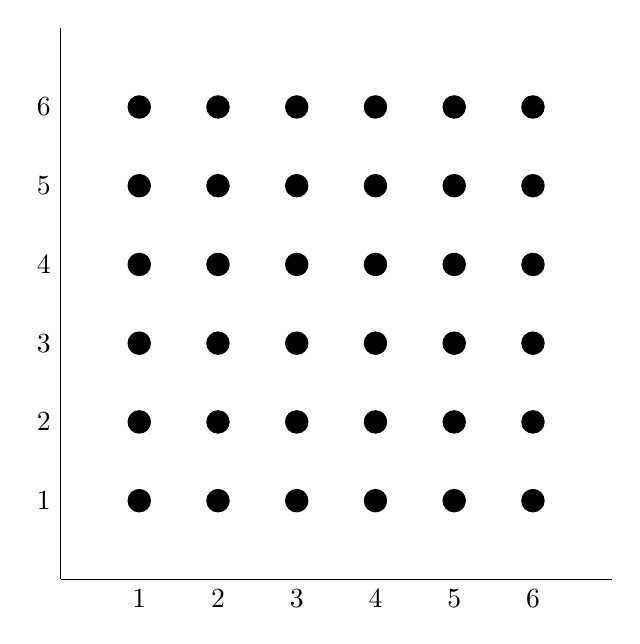
\begin{tikzpicture}[scale=1]
            \foreach \x in {1,...,6}
                {
                    \foreach \y in {1,...,6}
                        {
                            \node at (\x, \y)[circle,fill,inner sep=3pt]{};
                        }
                    \node[left] at (0, \x){$\x$};
                    \node[below] at (\x, 0){$\x$};
                }

            \draw (0.0, 0.0) -- (7.0, 0.0);
            \draw (0.0, 0.0) -- (0.0, 7.0);
        \end{tikzpicture}
    \end{center}

    为了证明这个格上无限多顶点是\textbf{可数}无限的,我们可以描述一条路径,该路径遍历所有的点(满射!)且每个点只遍历一次(单射!),并用自然数进行索引(可数无限!)。也就是说,我们可以描述一种通过一系列步骤遍历整个格上顶点的方式;会有一个``第一个点''和一个``第二个点''等等。

    关键的洞察是,这个格的左上对角线都是\textbf{有限的}。例如,从点 $(5, 1)$ 开始,向左上对角移动。你将经过 $(4, 2), (3, 3), (2, 4), (1, 5)$,然后到达格的边界。不论你从底部的哪一行开始,这都是正确的。

    让我们利用这一事实,根据 (a) 它所在的对角线,以及 (b) 它在该对角线上的位置,用自然数标记每个点。我们将从 $(1, 1)$ 开始的对角线视为第一条对角线,将从 $(2, 1)$ 开始的对角线视为第二条对角线,依此类推。这给了我们以下标注:

    \begin{center}
        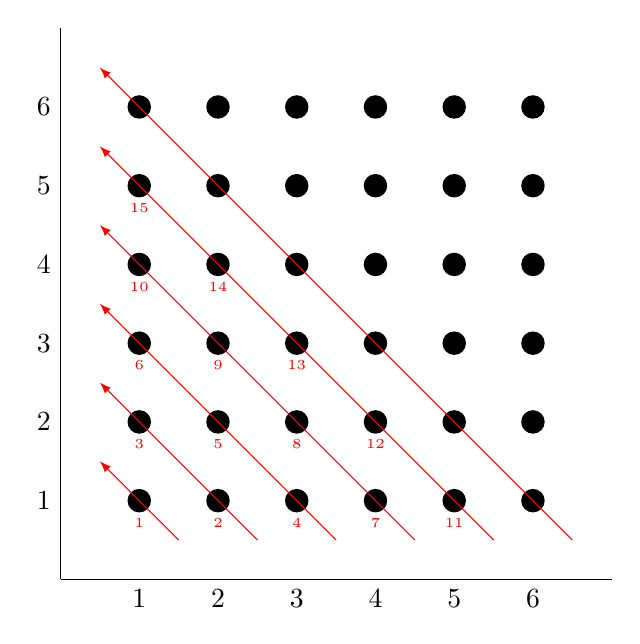
\begin{tikzpicture}[scale=1]
            \foreach \x in {1,...,6}
                {
                    \foreach \y in {1,...,6}
                        {
                            \node at (\x, \y)[circle,fill,inner sep=3pt]{};
                        }
                    \node[left] at (0, \x){$\x$};
                    \node[below] at (\x, 0){$\x$};
                    \draw[-latex, red] (\x+0.5, 0.5) -- (0.5, \x+0.5);
                }

            \draw (0.0, 0.0) -- (7.0, 0.0);
            \draw (0.0, 0.0) -- (0.0, 7.0);

            \foreach \y / \t in {1/1, 2/3, 3/6, 4/10, 5/15}
                {
                    \node[below,red] at (1, \y-0.1){\tiny$\t$};
                }
            \foreach \y / \t in {1/2, 2/5, 3/9, 4/14}
                {
                    \node[below,red] at (2, \y-0.1){\tiny$\t$};
                }
            \foreach \y / \t in {1/4, 2/8, 3/13}
                {
                    \node[below,red] at (3, \y-0.1){\tiny$\t$};
                }
            \foreach \y / \t in {1/7, 2/12}
                {
                    \node[below,red] at (4, \y-0.1){\tiny$\t$};
                }
            \node[below,red] at (5, 0.9){\tiny$11$};

        \end{tikzpicture}
    \end{center}

    我们可以看到,格中的每个顶点都会恰好落在某条对角线上。此外,这些对角线的数量是可数无限的(由 $\mathbb{N}$ 索引),而每条对角线上只有\emph{有限}多个点。这意味着(我们将在下面证明)所有对角线上的点的集合是可数无限集。

    你可以尝试通过定义一个函数来实现我们展示的标记方法,从而\emph{形式化}这个论点。或者,你也可以使用类似的方法,比如向右下方向移动,或者交替反转对角线的方向……
\end{example}

\begin{example}[$\mathbb{Q}$ 是可数无限集]

    这个结果是我们在处理无限集及其基数时,直觉失灵的一个显著例子。想象一下,把 $\mathbb{Q}$ 的元素分布在数轴上。它们似乎无处不在!事实上,回看练习 \ref{exc:exercises4.11.26},在那道练习中,你证明了有理数是\textbf{稠密的},这意味着在 $\mathbb{R}$ 中也是如此(即任意两个不同实数之间都存在一个有理数)。此外,有理数集\emph{看起来}比整数集 $\mathbb{Z}$ 大得多:仅在 $0$ 和 $1$ 之间,就有无穷多个有理数!出于这些原因,你可能会认为 $\mathbb{Q}$ 是不可数无限集,但这是错误的。

    在这个例子中,我们将提供几个论证来证明这一点,因为我们意识到这个结论确实非常奇特和炸裂。

    \begin{enumerate}[label=(\arabic*)]
        \item \textbf{直观解释:}\\
              考虑以下将 $\mathbb{Q}$ 表示为集合并集的形式:
              \[\mathbb{Q} \;\text{``}=\text{''}\; \big(\text{``}\mathbb{N} \times \mathbb{N}\text{''}\big) \cup \big(\text{``}-(\mathbb{N} \times \mathbb{N})\text{''}\big) \cup \{0\}\]
              某种意义上,$\mathbb{N} \times \mathbb{N}$ 可以对应所有正有理数。要理解这一点,只需考虑函数 $f : \mathbb{N} \times \mathbb{N} \to \mathbb{Q}_+$,定义为 $f(x, y) = \frac{x}{y}$。这个函数确实能够生成所有正有理数(因此 $f$ 是一个满射),但由于 $\frac{4}{2}=\frac{2}{1}$,所以它不是一个单射。因为 $f$ 是满射,这至少表明 $|\mathbb{N} \times \mathbb{N}| \ge |\mathbb{Q}|$。由于 $\mathbb{N} \times \mathbb{N}$ 是可数无限集,而 $\mathbb{Q}$ 显然也是无限集,这表明正有理数是可数无限集。\\

              负有理数集 $\mathbb{Q}_-$ 也具有与正有理数集 $\mathbb{Q}_+$ 相同的基数。它们之间存在明确的双射关系:定义函数 $g : \mathbb{Q}_+ \to \mathbb{Q}_-$ 为 $\forall q \in \mathbb{Q}_+ \centerdot g(q) = -q$。\\

              这里唯一遗漏的是 $0 \in \mathbb{Q}$。两个可数无穷集的并集仍然是可数无穷集(我们将在下面证明),再加上一个元素也不会改变这一点。因此,$\mathbb{Q}$ 是可数无限集。\\

              需要注意的是,这里有点``随意''。上面``等式''中的所有``引号''表示你应该仅将其作为启发性论证,而不是严格证明。然而,确实有方法可以使这些论证形式化。试着自己动手做做看吧!\\
        \item \textbf{列出 $\mathbb{Q}$ 中元素:}\\
              考虑编写一个计算机程序,列出所有正有理数。你会使用什么算法?只要你能保证你的程序``最终''会成功列出所有这些数,那么你就已经证明了 $\mathbb{Q}$ 可以一个一个地枚举出来,因此它必然是可数无限集。(这也是为什么我们使用 $\mathbb{N}$ 作为典型的可数无限集:我们可以一个一个地枚举它的元素,我们可以数它们。)\\

              这里有一种方法可以编写该程序:按照我们在前一个例子中使用 $\mathbb{N} \times \mathbb{N}$ ``格点路径''论证。这次,只需``跳过''已经打印过的有理数。\\

              也就是说,我们会先打印 $(1, 1) \leftrightarrow 1$,然后是 $(2, 1) \leftrightarrow 2$,再然后是 $(1, 2) \leftrightarrow \frac{1}{2}$,接着是 $(3, 1) \leftrightarrow 3$,依此类推……\\

              哦!我们需要跳过 $(2, 2) \leftrightarrow 1$。我们怎么知道的?因为我们已经打印过 $1$。我们怎么知道某个数已经打印过了?我们只需查看已经打印过的有理数列表,检查即将打印的数是否已经出现过。如果已经出现过,就跳过;如果没有,就打印它然后继续。\\

              在枚举过程中,这意味着对于我们经过的每个格点,我们只需检查\emph{有限的}项;也就是说,我们需要查看已经打印过的\emph{有限大的}有理数集合。这意味着在每一步打印过程中会花费``稍长一点的时间'',但不会\emph{无限长}。因此,我们的程序最终会列出每一个有理数;无论你想到的是哪个,我们都会在有限的时间内到达它。\\
        \item \textbf{$\mathbb{Q}$ 至多是可数无限集:}\\
              这是 $\mathbb{Q}$ 是可数集的另一个论证。(如果你觉得有点多余,那也没关系,可以跳过。我们只是觉得这个结果很有趣,从多个角度思考问题可能会有所帮助!)\\

              请思考一下:我们可以先验地认为 $|\mathbb{Q}| \ge |\mathbb{N}|$。这是因为 $\mathbb{Q} \supseteq \mathbb{N}$。现在,唯一的问题是这些基数是否相等。为了得出这个结论,我们需要找到
              \begin{enumerate}[label=(\alph*)]
                  \item 从 $\mathbb{Q}$ 到某个可数集的单射;
                  \item 从某个可数集到 $\mathbb{Q}$ 的满射。\\
              \end{enumerate}

              我们将在下面证明 $\mathbb{Z} \times \mathbb{N}$ 是可数的。(也就是说,我们将证明任意两个可数无限集的笛卡尔积也是可数无限集。)然后我们可以定义函数 $f : \mathbb{Z} \times \mathbb{N} \to \mathbb{Q}$ 为
              \[\forall (z, n) \in \mathbb{Z} \times \mathbb{N} \centerdot f(z, n) = \frac{z}{n}\]
              该函数是 $\mathbb{Q}$ 上的满射。虽然它肯定不是单射(为什么不是?)但这并不影响我们的结论。它表明 $|\mathbb{Z} \times \mathbb{N}| = |\mathbb{Q}|$。一旦我们证明了 $|\mathbb{Z} \times \mathbb{N}| = |\mathbb{N}|$,就可以得出 $|\mathbb{N}| = |\mathbb{Q}|$。\\
        \item \textbf{Stern-Brocot 树:}\\
              $\mathbb{Q}$ 还有其他视觉表示方法,其中 \textbf{Stern-Brocot 树}尤其具有启发性。这个概念最早由法国钟表匠 Achille Brocot 提出并发展,他在制作钟表时需要找到齿轮齿数的近似值。大约在同一时期($19$ 世纪 $50$ 年代和 $60$ 年代),德国数学家 Moritz Stern 也发展了这一想法。令人惊讶的是,一位非数学家竟然能\emph{独立地}发展出这样一个迷人的概念来解决实际问题!\\

              (不必过于担心\emph{图}和\emph{树}等术语。我们不会深入讨论它们,只是简单介绍一下,帮助理解 $\mathbb{Q}$ 的表示方法,并展示它是可数无穷集。)\\

              这棵树的\textbf{根节点}为 $1$。(即图中最顶端的数字。)\textbf{父节点和子节点的关系}(即如何生成树的下一层节点)是通过连分数定义的。(我们在这里不详细解释其含义,而是描述如何构建这棵树。)\\

              通过这种构造方法,从根节点到任一节点的路径会产生一系列有理数,这些有理数逐渐逼近最终的节点。此外,序列中的每个后续有理数的分母都比前一个大。这正是 Brocot 先生的动机所在。他需要确定手表内部两个齿轮的齿数,使它们的大小比率非常接近某个特定数值。通过沿着这棵树向下寻找,他可以找到更接近所需数值的近似比率!是不是很酷?

              \begin{center}
                  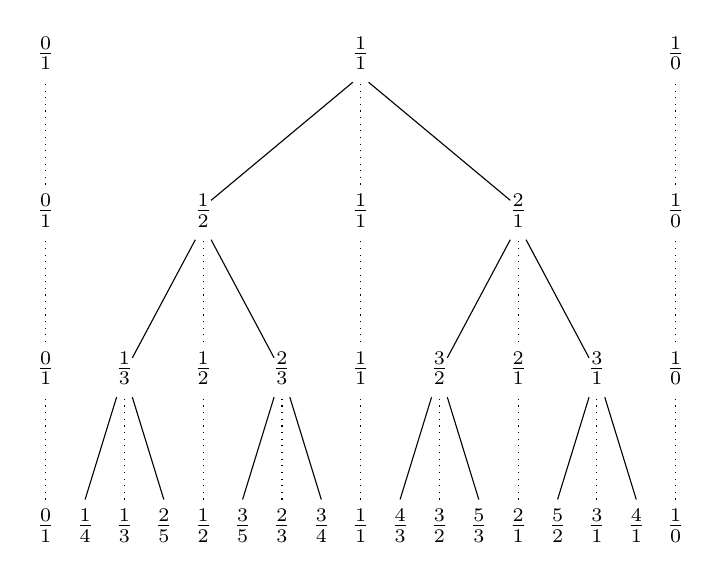
\begin{tikzpicture}[scale=1]
                      \edef \step {0.5};
                      \foreach \a / \b in {1/4, 1/3, 2/5, 1/2, 3/5, 2/3, 3/4}
                          {
                              \node[below] at (\step, 0){$\frac{\a}{\b}$};
                              \node[below] at (8-\step, 0){$\frac{\b}{\a}$};
                              \pgfmathparse{\step + 0.5};
                              \xdef \step{\pgfmathresult};
                          }

                      \edef \step {1.0};
                      \foreach \a / \b in {1/3, 1/2, 2/3}
                          {
                              \node[below] at (\step, 2){$\frac{\a}{\b}$};
                              \node[below] at (8-\step, 2){$\frac{\b}{\a}$};
                              \pgfmathparse{\step + 1.0};
                              \xdef \step{\pgfmathresult};
                          }

                      \node[below] at (2, 4){$\frac{1}{2}$};
                      \node[below] at (6, 4){$\frac{2}{1}$};

                      \foreach \y in {0,...,3}
                          {
                              \node[below] at (0, \y*2){$\frac{0}{1}$};
                              \node[below] at (4, \y*2){$\frac{1}{1}$};
                              \node[below] at (8, \y*2){$\frac{1}{0}$};
                          }

                      \edef \mx {0.1};
                      \edef \mya {0.2};
                      \edef \myb {0.7};
                      \foreach \y in {0,...,2}
                          {
                              \draw[dotted] (4, \y*2) -- (4, \y*2 + 2-\myb);
                          }

                      \foreach \x in {0,...,3}
                          {
                              \draw[dotted] (\x, 0.0) -- (\x, 2-\myb);
                              \draw[dotted] (8-\x, 0.0) -- (8-\x, 2-\myb);
                              \draw (\x*2+0.5, 0.0) -- (\x*2+1-\mx, 2-\myb);
                              \draw (\x*2+1.5, 0.0) -- (\x*2+1+\mx, 2-\myb);
                          }
                      \foreach \x in {0,...,1}
                          {
                              \draw[dotted] (\x*2, 2.0) -- (\x*2, 4-\myb);
                              \draw[dotted] (8-\x*2, 2.0) -- (8-\x*2, 4-\myb);
                              \draw (\x*4+1+\mx, 2.0-\mya) -- (\x*4+2-\mx, 4-\myb);
                              \draw (\x*4+3-\mx, 2.0-\mya) -- (\x*4+2+\mx, 4-\myb);
                          }
                      \foreach \x in {0}
                          {
                              \draw[dotted] (\x*8, 4.0) -- (\x*8, 6-\myb);
                              \draw[dotted] (8-\x*8, 4.0) -- (8-\x*8, 6-\myb);
                              \draw (\x*8+2+\mx, 4.0-\mya) -- (\x*8+4-\mx, 6-\myb);
                              \draw (\x*8+6-\mx, 4.0-\mya) -- (\x*8+4+\mx, 6-\myb);
                          }
                  \end{tikzpicture}
              \end{center}

              为了实际\emph{构建}这棵树,我们需要找到\emph{中位数}。给定两个有理数 $\frac{a}{b}$ 和 $\frac{c}{d}$,它们的中位数定义为 $\frac{a+b}{c+d}$。(注意,这里的中位数指的是一种特殊的对象;这\emph{不是}两个分数相加的正确方法!)\\

              树的每一层由上一层中相邻有理数对的所有中位数组成;我们不``计算''直接垂直的元素,它们只是为了便于阅读和构建而保留的。此外,注意分数 $\frac{0}{1}$ 和 $\frac{1}{0}$(尽管 $\frac{1}{0}$ 是未定义的!)包含在外侧列中,用于辅助生成每层最外侧的元素。\\

              (可以尝试探索这棵树的性质,并阅读更多\href{https://en.wikipedia.org/wiki/Stern%E2%80%93Brocot_tree}{相关内容}。这是一个非常有趣的数学对象!)\\

              我们在这里不会证明这棵树包含\emph{所有}有理数,但我们相信你可以理解为什么这是可信的。此外,我们也相信你可以理解为什么这棵树中的所有节点集合是\textbf{可数}无限集。每一层只有有限多个节点,而层数是可数无穷多层。
    \end{enumerate}

\end{example}

\subsubsection*{定理}

现在我们知道,$\mathbb{N}, \mathbb{Z}, \mathbb{Q}$ 这三个标准数集,以及 $\mathbb{N} \times \mathbb{N}$,都是可数无限集。接下来,通过一些定理,我们将展示如何从这些已有集合中生成更多的可数无限集。

我们先来看一个有用的结论。这个结论表明,如果我们在一个可数无限集上``添加''有限多个元素,结果仍然是可数无限集。

\begin{lemma}\label{lemma7.6.16}
    如果 $A$ 是可数无限集,$B$ 是有限集且 $A \cap B = \varnothing$,则 $A \cup B$ 为可数无限集。
\end{lemma}

\begin{proof}
    留作练习 \ref{exc:exercises7.8.19}

    (\textbf{提示}:采用与证明定理 \ref{theorem7.6.7} 类似的思路。)
\end{proof}

\begin{remark}
    注意:在这个引理中,假设 $A \cap B = \varnothing$ 并非\emph{必要},但它可以简化证明过程。

    当 $A \cap B \ne \varnothing$ 时,我们可以将刚刚证明的结果应用到集合 $A - B$(它是可数无限集)和 $B - A$(它是有限集)上,从而得到可数无限的集 $(A - B) \cup (B - A)$(因为它们是互斥的)。然后,我们可以再次将上述结论应用于该集合 --- $(A - B) \cup (B - A)$ --- 和 $A \cap B$,从而得到可数无限集:
    \[A \cup B = (A - B) \cup (B - A) \cup (A \cap B)\]
\end{remark}

下一个结论表明,该方法同样适用于 $A$ 和 $B$ 都是可数无限集的情况。

\begin{lemma}\label{lemma7.6.18}
    如果 $A$ 和 $B$ 都是可数无限集,且 $A \cap B = \varnothing$,则 $A \cup B$ 为可数无限集。
\end{lemma}

\begin{proof}
    因为 $A$ 和 $B$ 为可数无限集,则存在双射 $ f : A \to \mathbb{N}$ 和 $g : B \to \mathbb{N}$。给定这样的函数,我们要找到 $h : A \cup B \to \mathbb{N}$。

    首先定义函数 $p : \mathbb{N} \to \mathbb{Z} - \mathbb{N}$ 为 $\forall n \in \mathbb{N} \centerdot p(n) = -n + 1$。

    这是一个双射,因为 $p^{-1} : \mathbb{Z} - \mathbb{N} \to \mathbb{N}$ 为 $p^{-1}(z) = -z + 1$。(请你自行验证!)

    由于 $p$ 和 $g$ 都是双射,所以 $p \circ g : \mathbb{Z} - \mathbb{N}$ 也为双射。

    接着我们定义分段函数 $q : A \cup B \to \mathbb{Z}$ 为
    \[\forall x \in A \cup B \centerdot q(x) = \begin{cases}
            f(x)    & \text{如果}\; x \in A \\
            p(g(x)) & \text{如果}\; x \in B
        \end{cases}\]
    这是一个良好定义的函数,因为 $A \cap B = \varnothing$。此外,这也是一个双射函数,因为每一段函数都是双射。(请你自行检验以确保它是合理的。另外,请参见练习 \ref{exc:exercises7.8.31},那里给出了一般情况下的证明。)

    综上,我们知道如何构建双射 $r : \mathbb{Z} \to \mathbb{N}$。(还记得我们是怎么做的吗?请参考示例 \ref{ex:example7.6.12}。)

    最后,定义函数 $h : A \cup B \to \mathbb{N}$ 为 $h = r \circ q$。这个函数是双射的复合,因此也是双射。这证明了 $ |A \cup B| = |\mathbb{N}|$,即 $A \cup B$ 为可数无限集。
\end{proof}

接下来的推论表明,实际上我们不需要假设 $A \cap B = \varnothing$。这个假设只是为了让证明过程更简单。我们希望你能证明这个推论。

\begin{corollary}\label{corollary7.6.19}
    如果 $A$ 和 $B$ 都是可数无限集,则 $A \cup B$ 为可数无限集。
\end{corollary}

\begin{proof}
    留作练习 \ref{exc:exercises7.8.20}。

    (\textbf{提示}:将引理 \ref{lemma7.6.18} 应用于适当的集合上……)
\end{proof}

以上证明了几个关于集合\emph{并集}的情况。接下来我们来证明一个关于\emph{笛卡尔积}的结论。

\begin{theorem}
    如果 $A$ 和 $B$ 都是可数无限集,则 $A \times B$ 为可数无限集。
\end{theorem}

这个证明其实很简单,因为我们已经证明了关于 $\mathbb{N} \times \mathbb{N}$ 结论。这个集合是笛卡尔积,并且是可数无穷集。请看我们在证明中如何使用 $\mathbb{N} \times \mathbb{N}$:

\begin{proof}
    假设 $A$ 和 $B$ 为可数无限集,则存在双射 $ f : A \to \mathbb{N}$ 和 $g : B \to \mathbb{N}$。给定这样的函数。

    定义函数 $h : A \times B \to \mathbb{N} \times \mathbb{N}$ 为
    \[\forall (x, y) \in A \times B \centerdot h(x, y) = \big(f(x), g(y)\big)\]
    我们声称这是一个双射函数。因为 $f, g$ 都是可逆的,定义函数 $H : \mathbb{N} \times \mathbb{N} \to A \times B$ 为
    \[\forall (k, \ell) \in \mathbb{N} \times \mathbb{N} \centerdot H(k, \ell) = \big(f^{-1}(k), g^{-1}(\ell)\big)\]
    我们声称 $H = h^{-1}$。因为
    \begin{align*}
        \forall (x, y) \in A \times B \centerdot (H \circ h)(x, y) & = H(h(x, y)) = H \big(f(x), g(y)\big)           \\
                                                                   & = \big(f^{-1}(f(x)), g^{-1}g((y))\big) = (x, y)
    \end{align*}
    且
    \begin{align*}
        \forall (k, \ell) \in \mathbb{N} \times \mathbb{N} \centerdot (h \circ H)(k, \ell) & = h(H(k, \ell)) = h\big(f^{-1}(k), g^{-1}(\ell)\big)  \\
                                                                                           & = \big(f(f^{-1}(k)), g(g^{-1}(\ell))\big) = (k, \ell)
    \end{align*}
    所以 $H \circ h = \id_{A \times B}$ 且 $h \circ H = \id_{\mathbb{N} \times \mathbb{N}}$。这表明 $H = h^{-1}$。

    因此,$h$ 为双射。所以 $|A \times B| = |\mathbb{N} \times \mathbb{N}| = |\mathbb{N}|$。
\end{proof}

通过对前两个结论进行归纳,我们可以证明以下推论:

\begin{corollary}\label{corollary7.6.21}
    假设 $A_1, \dots , A_n$ 为可数集(其中 $n \in \mathbb{N}$,所以我们有可数无限个集合),则 $A_1 \cup \dots \cup A_n$ 和 $A_1 \times \dots \times A_n$ 为可数无限集
\end{corollary}

\begin{proof}
    留作练习 \ref{exc:exercises7.8.22}。
\end{proof}

\subsubsection*{可数个可数集的并集为可数集}

你可能会好奇,当我们对\emph{可数无穷多}个集合(每个集合都是可数无限集)进行并集或乘积运算时,会发生什么情况。让我们先来探讨并集的情况。这个结果非常基础且重要,我们甚至在章节标题中重复强调了它!

\begin{theorem}\label{theorem7.6.22}
    对于每个 $n \in \mathbb{N}$,假设我们有 $A_n$ 为可数无限集,则集合
    \[A = \bigcup_{n \in \mathbb{N}} A_n = A_1 \cup A_2 \cup A_3 \cup \dots\]
    为可数无限集。
\end{theorem}

我们将证明集合\textbf{互不相交}的情况,剩下的细节留给你来处理。

\begin{proof}
    对于每个 $n \in \mathbb{N}$,假设我们有 $A_n$ 为可数无限集,且 $\forall i, j \in \mathbb{N} \centerdot i \ne j \implies A_i \cap A_j = \varnothing$。定义
    \[A = \bigcup_{n \in \mathbb{N}} A_n\]
    我们声称 $A$ 为可数无限集。

    因为每一个 $A_n$ 都是有限可数集,我们知道对于每一个 $n \in \mathbb{N}$ 存在双射 $f_n : A_n \to \mathbb{N}$。这使得我们能够根据双射 $f_n$ 的定义对每一个集合 $A_n$ 的元素进行``编号''。此外,我们对 $A_n$ 集合进行编号,这些集合由 $\mathbb{N}$ 索引。本质上,我们对 $A$ 的元素进行了``编号'',这些编号对应于 $\mathbb{N} \times \mathbb{N}$。接下来我们将正式定义这种对应关系。

    我们定义函数 $F : A \to \mathbb{N} \times \mathbb{N}$。给定任意 $x \in A$,我们知道 $\exists n \in \mathbb{N} \centerdot x \in A_n$ 且 $n$ 是\emph{唯一的}。(这是因为给定的集合是互不相交的)。设 $F(x) = \big(n, fn(x)\big)$。

    我们声称 $F$ 为双射。考虑函数 $G : \mathbb{N} \times \mathbb{N} \to A$ 定义为
    \[\forall (a, b) \in \mathbb{N} \times \mathbb{N} \centerdot G(a, b) = f_a^{-1}(b)\]
    也就是说,$G$ 使用第一个坐标 $a$ 来确定集合 $A_a$,然后使用函数 $f_a$ 来确定 $A_a$ 中输出 $b \in \mathbb{N}$ 的元素。

    (留给读者验证 $G = F^{-1}$。)

    这表明 $|A| = |\mathbb{N} \times \mathbb{N}| = |\mathbb{N}|$,所以 $A$ 是可数无限集。

    $A_n$ 可能相交的情况,留作练习 \ref{exc:exercises7.8.37}。
\end{proof}

\begin{corollary}\label{corollary7.6.23}
    对于每个 $n \in \mathbb{N}$,假设我们有 $A_n$ 为有限集,且这些集合互不相交。定义集合
    \[A = \bigcup_{n \in \mathbb{N}} A_n\]
    则 $A$ 为可数有限集。
\end{corollary}

\begin{proof}
    留作练习 \ref{exc:exercises7.8.36}。
\end{proof}

这个结论非常强大。让我们两个应用示例。\\

\begin{example}[所有质数幂次的集合]
    还记得希尔伯特旅馆的讨论吗?在那个例子中,我们容纳了无穷多个会议,每个会议的人数也是无穷的。我们将客人们安排到对应质数幂次的房间。对于每一个 $n \in \mathbb{N}$,定义 $p_n$ 为第 $n$ 个质数。则
    \[A_n = \{p_n^k \mid k \in \mathbb{N}\}\]
    为第 $n$ 个质数所有幂次的集合。上面的定理告诉我们
    \[\bigcup_{n \in \mathbb{N}} A_n = \{\text{质数的所有幂次}\}\]
    也是可数无限集。确实,这并不意外,因为上面的并集只是自然数的一个子集,而自然数本身是可数无限集!
\end{example}

\begin{example}[所有有限长二进制字符串的集合]\label{ex:example7.6.25}
    二进制字符串被定义为由 \verb|0| 和 \verb|1| 组成的有序序列。\textbf{有限长二进制字符串}是指长度有限的二进制字符串。

    例如,下面这些都是有限长二进制字符串:
    \[0, \quad 1, \quad 101010, \quad 10000000000000000001 \]

    对于每个 $n \in \mathbb{N}$,定义 $F_n$ 为所有长度为 $n$ 的二进制字符串的集合。例如
    \begin{align*}
        F_1 & = \{ 0 , 1 \}                                         \\
        F_2 & = \{ 00 , 01 , 10 , 11 \}                             \\
        F_3 & = \{ 000 , 001 , 010 , 100 , 011 , 101 , 110 , 111 \}
    \end{align*}
    依此类推。(注意 $|F_n| = 2^n$。试着证明一下。)则定义所有有限长二进制字符串的集合为
    \[F = \bigcup_{n \in \mathbb{N}} F_n\]

    $F$ 的每个元素必须来自大并集中的某个集合;这意味着任意元素 $x \in F_n$ 都是某个具有有限长度的二进制字符串。这个长度可能非常大,但它是有限的。(这说明了``任意大(但有限)''和``无限''之间的区别。)

    这个例子的重点是,根据上面的定理,$F$ 是可数的!(实际上,这是从紧随其后的推论得出的。)相比之下,所有\emph{无限长}二进制字符串的集合 $S$ 是不可数的 --- 我们很快会证明这一点。我们将经常使用这些二进制字符串集合作为例子!
\end{example}

\subsubsection*{取``极限''}

我们已经证明,如果 $A$ 和 $B$ 是可数无限集,那么 $A \cup B$ 和 $A \times B$ 也是可数无限集。我们还建议你使用归纳法(对并集或乘积中的集合数量进行归纳)来证明,对于任意 $n \in \mathbb{N}$,
\[A_1 \cup A_2 \cup \dots \cup A_n = \bigcup_{i \in [n]} A_i \quad \text{和} \quad \prod_{i \in [n]} A_i = A_1 \times A_2 \times \dots \times A_n\] 
也是可数无限集。

这些结论是否为我们提供了某些关于
\[A_1 \cup A_2 \cup A_3 \cup \dots = \bigcup_{k \in \mathbb{N}} A_k\]
和
\[A_1 \times A_2 \times A_3 \times \dots = \prod_{k \in \mathbb{N}} A_k\]
的信息?也就是说,当我们尝试从\emph{有限}数量的并集/乘积(任意大但仍然有限)过渡到\emph{无限}数量的并集/乘积时,会发生什么?我们能得出必要的结论吗?我们能找到反例吗?

主要思想是,``取极限''确实会创建某些数学对象,但我们不能预先假设这个对象具有与定义它的序列中所有对象\emph{完全相同的属性}。

考虑有限集 $[n]$,对于每个 $n$,它们都是有限的,但``取极限''后我们得到的 $\mathbb{N}$ 是无限的。所以我们确实得到了一个对象(另一个集合),但它不一定具有相同的属性。

上述重要定理表明,在\emph{并集}中取极限肯定会保留可数性。正如我们将在下一节中看到的那样,\emph{乘积}肯定\textbf{不会}保留可数性。(实际上,即使是无限个有限集的乘积也是不可数的。真是令人惊讶!)

在微积分中也有类似的概念。我们本来承诺不使用微积分,但这些思想之间有如此自然的关系,所以我们不得不提及一个简单的例子。如果你不理解也没关系;如果你理解了,试着记住这个联系,并思考它如何从根本上改变了你在微积分中学到的一切。)

考虑如下\emph{极限}:
\[\lim_{x \to \infty} \frac{1}{x} = 0\]
这个极限在什么意义上\textbf{等于} $0$?为什么身为资深数学家的我们会选择用这种方式\emph{定义}极限?形式上,这个极限是有意义的,因为它符合极限的量化定义。设 $P$ 为正实数集,极限的定义(应用于这个例子)为
\[\forall \varepsilon \in P \centerdot \exists M \in \mathbb{N} \centerdot \forall n \in \mathbb{N} \centerdot \big(n > M \implies \big|\frac{1}{x}\big| < \varepsilon \big)\]
也就是说,对于任何小的正阈值($\varepsilon > 0$),我们都可以找到一个特定的截止点(一个依赖于 $\varepsilon$ 的大自然数 $M$),使得 $M$ \emph{之后}的每一点,函数 $\frac{1}{x}$ 都在极限点 $0$ 的 $\varepsilon$ 阈值内。

请注意,这与 ``$\frac{1}{\infty} = 0$'' 这样的说法\emph{完全不同}。事实并非如此。实际上,我们从未真正``代入''极限的终点来进行计算。极限是通过量化定义的,也就是说,我们讨论的是在\emph{任意大}值下发生的情况,而不是在\emph{无限大}值下发生的情况。

% !TeX root = ../../../book.tex

\subsection{不可数集}

在讨论不可数集之前,我们先证明一个先前提及的结果:集合的可数无限次\emph{笛卡尔积}是不可数的。值得注意的是,这些集合甚至不必是无限集——它们可以都是大小为 $2$ 的有限集。在下一节中,我们将利用这一结论展示一些不可数集的例子,包括一个我们熟知的集合……

\subsubsection*{不可数笛卡尔积}

\begin{theorem}
    双元素集合的可数无限次笛卡尔积是不可数的。即
    \[\{0, 1\}^{\mathbb{N}} = \{0, 1\} \times \{0, 1\} \times \{0, 1\} \times \dots\]
    是不可数无限集。
\end{theorem}

\begin{proof}
    为了引出矛盾而假设 $\{0, 1\}^{\mathbb{N}}$ 是可数无限集。这意味着存在该集合与 $\mathbb{N}$ 之间的双射,从而可以将集合中的每个元素与一个自然数一一对应。因此,该集合中的元素可以枚举为:第一个元素对应自然数 $1$,第二个对应 $2$,依此类推。

    尽管我们不知道这些元素的具体形式,但可以确认这样的对应关系一定存在。我们可以将 $\{0, 1\}^{\mathbb{N}}$ 的所有元素记为 $y_i$,其中每个 $y_i$ 是一个由 $0$ 和 $1$ 组成的无限序列,因此可以表示为:
    \begin{align*}
        1 & \leftrightarrow (a_{1,1} , a_{1,2} , a_{1,3} , a_{1,4} , a_{1,5} , \dots) = y_1 \\
        2 & \leftrightarrow (a_{2,1} , a_{2,2} , a_{2,3} , a_{2,4} , a_{2,5} , \dots) = y_2 \\
        3 & \leftrightarrow (a_{3,1} , a_{3,2} , a_{3,3} , a_{3,4} , a_{3,5} , \dots) = y_3 \\
        4 & \leftrightarrow (a_{4,1} , a_{4,2} , a_{4,3} , a_{4,4} , a_{4,5} , \dots) = y_4 \\
        5 & \leftrightarrow (a_{5,1} , a_{5,2} , a_{5,3} , a_{5,4} , a_{5,5} , \dots) = y_5 \\
          & \vdots
    \end{align*}
    每个值 $a_{i,j}$ 要么是 $0$,要么是 $1$。这里,$i$ 表示对应的自然数(即\emph{垂直}位置),$j$ 表示序列中的坐标(即\emph{水平}位置)。

    由于假设该对应关系是双射,所以上述列表包含了 $\{0, 1\}^{\mathbb{N}}$ 的所有元素。为了完成反证法,我们将构造一个 $\{0, 1\}^{\mathbb{N}}$ 中的元素,并证明它\textbf{不在}列表中。(这正是康托尔对角线论证的一种形式。)

    我们定义对象 $x = (x_1, x_2, x_3, \dots)$ 为
    \[x_i = \begin{cases}
            0 & \text{若}\; a_{i,i} = 1 \\
            1 & \text{若}\; a_{i,i} = 0
        \end{cases}\]
    也就是说,我们沿矩阵的\emph{主对角线}(考虑所有 $a_{i,i}$)构建 $x$,并将每个值\emph{取反},即 $1$ 变为 $0$,$0$ 变为 $1$。

    下图通过一个\emph{具体示例}说明这一过程(虽然它不是证明的必要部分,但有助于理解):
    \begin{align*}
        1 & \leftrightarrow (\circled{1} , 1 , 0 , 0 , 1 , \dots) = y_1                        \\
        2 & \leftrightarrow (1 , \circled{0} , 0 , 0 , 1 , \dots) = y_2                        \\
        3 & \leftrightarrow (0 , 0 , \circled{1} , 1 , 0 , \dots) = y_3                        \\
        4 & \leftrightarrow (1 , 1 , 0 , \circled{1} , 1 , \dots) = y_4                        \\
        5 & \leftrightarrow (0 , 1 , 1 , 1 , \circled{0} , \dots) = y_5                        \\
          & \vdots                                                                             \\
        x & =\left(\circled{0}, \circled{1}, \circled{0}, \circled{0}, \circled{1}, \dots \right)
    \end{align*}
    我们这样做的目的是什么?考虑 $x$ 是否可能出现在上述列表中。
    \begin{itemize}
        \item $x = y_1$ 吗?不相等!因为 $x$ 与 $y_1$ 的第一个坐标不同。(在本例中,$x_1=0$ 而 $y_{1,1} = 1$。)
        \item $x = y_2$ 吗?不相等!因为 $x$ 与 $y_2$ 的第二个坐标不同。(在本例中,$x_2=1$ 而 $y_{2,2} = 0$。)
        \item $x = y_3$ 吗?不相等!因为 $x$ 与 $y_3$ 的第三个坐标不同。(在本例中,$x_3=0$ 而 $y_{3,3} = 1$。)
    \end{itemize}
    一般来讲,对于任意 $i \in \mathbb{N}$,我们可以保证 $x$ 与 $y_i$ 在第 $i$ 个坐标上不同。因此,\textbf{没有}任何 $y_i$ 等于 $x$,即
    \[\left(\forall i \in \mathbb{N} \centerdot x_i \ne y_{i,i}\right) \implies \left(\forall i \in \mathbb{N} \centerdot x \ne yi\right)\]
    然而,根据定义,$x$ 是一个由 $0$ 和 $1$ 组成的无限序列,故 $x \in \{0, 1\}^{\mathbb{N}}$。

    这就产生了矛盾:我们假设可以列出集合中的所有元素,但随后我们用这种顺序构造了一个不在集合中的元素。$\hashx$

    因此,$\{0, 1\}^{\mathbb{N}}$ 为不可数无限集。
\end{proof}

请注意:这是一个非常巧妙的论证,也是我最喜欢的数学证明之一。康托尔真是个天才,他想出了这个证明;更有趣的是,这个证明实际上相当简单且令人难忘。我们相信你不会忘记这个``沿主对角线切换值''的论证。我们甚至可以用八个字总结整个证明,这进一步凸显了它的精彩。

请注意:这是一个非常巧妙的论证。这是我最喜欢的数学证明之一。康托尔真是个天才,他想出了这个证明,更有趣的是,这个证明实际上相当简单且令人难忘。我们相信你不会忘记这个``沿主对角线切换值''的论证。我们甚至可以用八个字总结整个证明,这进一步彰显了它的精彩。

\begin{corollary}
    对于任意至少包含两个元素的集合,其可数无限次笛卡尔积是不可数无限的。
\end{corollary}
(注意:实际上,我们只需乘积中的每个集合非空,且最多有有限个集合只有一个元素。)

\subsubsection*{示例}

你可能会好奇:什么样的集合是不可数无限的呢?我们知道这样的集合吗?当然!以下是一些例子。

\begin{example}[所有无限长二进制字符串的集合]

    你可能已经注意到,我们在上面证明中使用的集合——即 $\{0, 1\}^\mathbb{N}$——实际上就是无限长二进制字符串的集合 $S$!$\{0, 1\}^\mathbb{N}$ 中的元素是无限长有序序列,每个位置上的值都是 \verb|0| 或 \verb|1|。$S$ 中的元素也是由 \verb|0| 和 \verb|1| 组成的无限长有序序列,只是不包含括号和逗号。因此,这两者之间存在一个非常自然的双射关系(只需去掉括号和逗号,或者加上它们),所以我们将这两个集合视为相同集合。

    我们在上面的示例 \ref{ex:example7.6.25} 中看到,所有有限长二进制字符串的集合是可数无限集。如上所述,所有无限长二进制字符串的集合是不可数无限集。另一种证明这一事实的方法是找到 $S$ 与 $\mathcal{P}(\mathbb{N})$ 之间的双射,然后应用康托尔定理,该定理指出 $|\mathbb{N}| < |\mathcal{P}(\mathbb{N})|$。(详见练习 \ref{exc:exercises7.8.33}。)
\end{example}

\begin{example}[$\mathbb{R}$ 是不可数无限集]

    这是我们首次接触一个标准的不可数无限集。我们可以利用上述结论来证明这一点。

    直觉上,这个说法是合理的,因为实数轴看起来比自然数集 $\mathbb{N}$ 或整数集 $\mathbb{Z}$ 大得多。但我们也知道,有理数集 $\mathbb{Q}$ 是可数无限集,并且在实数轴上存在无数个有理数。实际上,\emph{在任意两个实数之间}都存在无限多个有理数。
    
    我们将看到,实数集 $\mathbb{R}$ 确实是不可数无限集。此外,我们还将证明 $\mathbb{R}$ 与幂集 $\mathcal{P}(\mathbb{N})$ 具有相同的``无限大小'';也就是说,我们将证明 $|\mathbb{R}| = |\mathcal{P}(\mathbb{N})|$。(请记住,这比仅仅说两个集合都是不可数集包含更多信息;不可数无限集有许多级别,我们暂时不深入讨论,以免头脑爆炸。)

    直观上,要理解 $\mathbb{R}$ 是不可数无限集,可以先将 $\mathbb{R}$ 与集合 $\{0, 1, 2, 3, 4, 5, 6, 7, 8, 9\}^\mathbb{N}$ 关联起来。每个实数都可以用十进制表示,这实际上是一个有序的、可数无限的数字序列。尽管在十进制表示中会出现像 $0.999999 \dots = 1$ 这样的问题,但这些并不影响主要结论。既然我们已经知道,即使像 $\{0, 1\}$ 这样的小集合,在无限次取积时也会生成一个不可数集合,那么对于更大的集合,如 $\{0, 1, \dots, 9\}$,也必定会生成一个不可数集合。这个直观的论证可以帮助你理解并向朋友解释这一结论。(事实上,大多数教科书也是这样解释的。)

    更正式地,我们可以证明 $|\mathbb{R}| = |\mathcal{P}(\mathbb{N})|$。这个更强的结论意味着 $\mathbb{R}$ 是不可数无限集(因为康托尔定理指出 $|\mathbb{N}| < |\mathcal{P}(\mathbb{N})|$)。为此,我们考虑集合
    \[I = \{y \in \mathbb{R} \mid 0 \le y \le 1\}\]
    即区间 $[0, 1] \subseteq \mathbb{R}$。我们将证明
    \[|{0, 1}^\mathbb{N}| = |\mathcal{P}(\mathbb{N})| = |I|\]
    然后再应用一些关于区间与 $\mathbb{R}$ 之间存在双射的结论。

    考虑函数 $f_1 : \{0, 1\}^{\mathbb{N}} \to I$,它接受一个无限长二进制字符串,在字符串前加上一个小数点,并将其解释为\textbf{十进制}表示。

    例如,考虑元素 $(1, 1, 0, 0, 1, 0, \dots)$,其余部分为 $0$。则
    \[f_1(1, 1, 0, 0, 1, 0, \dots) = 0.110010 \dots _\text{DEC} = \frac{1}{10^1}+\frac{1}{10^2}+\frac{1}{10^5} = \frac{11001}{100000}\]
    请注意,这确实是一个函数,因为任何输出都是一个实数(因为它有小数表示;我们刚刚给出了一个例子),并且其值介于 $0$ 和 $1$ 之间,因为我们在最前面加了小数点。此外,函数 $f_1$ 是\textbf{单射};两个不同的无限长二进制字符串在某些位置上必然不同,因此它们表示的小数在某些位上也不同,从而不可能是相同的实数。这表明 $|\{0,1\}^{\mathbb{N}}| \le |I|$。

    考虑函数 $f_2 : \{0, 1\}^{\mathbb{N}} \to I$,它接受一个无限长二进制字符串,在字符串前加上一个小数点,并将其解释为\textbf{二进制}表示。

    例如,考虑上述相同元素。则
    \[f_2(1, 1, 0, 0, 1, 0, \dots) = 0.110010 \dots _\text{BIN} = \frac{1}{2^1}+\frac{1}{2^2}+\frac{1}{2^5} = \frac{25}{32}\]
    请注意,这确实是一个函数,因为任何输出都是一个实数;只需计算分数求和,就会得到一个介于 $0$ 和 $1$ 之间的实数(即使序列是无限的,它也保证收敛)。例如,当输入全为 $0$ 时,输出为 $0$;当输入全为 $1$ 时,输出为 $1$,因为
    \[\frac{1}{2}+\frac{1}{4}+\frac{1}{8}+\dots = \sum_{k \in \mathbb{N}} \frac{1}{2^k} = 1\]
    此外,函数 $f_2$ 是\textbf{满射}。这一事实依赖于一些关于有理数和无理数的外部知识;具体来说,任何无理数都可以通过一系列二进制有理数(即分母为 $2$ 的幂的有理数)来逼近。我们不会详细阐述或证明这些结论,但我们认为通过一些例子,你会逐渐理解其原理。事实上,搜索无理数的二进制展开,你会发现一些有趣的结果。

    因为 $f_2$ 是满射,这表明 $|\{0,1\}^{\mathbb{N}}| \ge |I|$。综上,我们得出结论 $|\{0,1\}^{\mathbb{N}}| = |I|$。我们还知道 $|\mathcal{P}(\mathbb{N})| = |\{0, 1\}^{\mathbb{N}}|$(见练习 \ref{exc:exercises7.8.33}),所以我们知道 $|I| = |\mathcal{P}(\mathbb{N})|$。

    最后一步是证明 $|I| = |\mathbb{R}|$。回看 \ref{sec:section7.5.4} 节中的练习 \ref{exc:exercises7.5.5}。在那里我们找到了集合 $J = \{y \in \mathbb{R} \mid -1 < y < 1\}$ 和 $\mathbb{R}$ 之间的双射。很容易找到集合 $J$ 与集合 $K = \{y \in \mathbb{R} \mid 0 < y < 1\}$ 之间的双射(不妨现在试一试!)。这表明 $|\mathbb{R}| = |J| = |K|$。此外,$K \subseteq I$,它们之间唯一的区别在于元素 $0$ 和 $1$,因此 $|K| = |I|$。最终,我们证明了 $|I| = |\mathbb{R}|$。因此,我们可以得出如下结论:
    \[|\mathbb{R}| = |\mathcal{P}(\mathbb{N})|\]
    我们回顾一下之前提到的两个论证:
    \begin{itemize}
        \item 考虑集合 $\{0, 1, 2, 3, 4, 5, 6, 7, 8, 9\}^\mathbb{N}$
        \item 考虑集合 $\{0, 1\}^\mathbb{N}$
    \end{itemize}
    这两个论证都涉及一些关于十进制展开和二进制展开的知识。似乎没有简单的方法绕过这一点,因此我们希望上述结果仍然是令人信服的。特别是,你可以思考上面讨论中 $f_2$ 是\textbf{满射}但不是\textbf{单射}的结论。你能说服自己接受这个观点吗?你能说服他人吗?
\end{example}

\subsubsection*{定理}

我们首先介绍一个关于不可数集的结论,随后陈述一个关于无限集的最终定理。。

\begin{lemma}\label{lemma7.6.29}
    假设 $A$ 为不可数无限集,$B$ 为可数无限集,且 $B \subseteq A$。则 $A-B$ 为不可数无限集。
\end{lemma}

(注意:我们\emph{不需要}假设 $B \subseteq A$。如果 $B \not\subseteq A$,可以考虑集合 $A$ 和 $B \cap A$。)

\begin{proof}
    留作 \ref{sec:section7.6.5} 节的练习 \ref{exc:exercises7.6.5}。

    (\textbf{提示}:采用反证法……)
\end{proof}

\subsubsection*{识别无限集}

为了定义\textbf{无限集},我们首先定义了\textbf{有限集},然后称任何\emph{不是}有限集的集合为无限集。下面的定理提供了另一种定义\textbf{无限集}的方式:一个集合是无限集,当且仅当存在一个双射将其映射到自身的一个真子集。首先,我们陈述并证明一个有用的引理,该引理将在后续定理的证明中发挥作用。

\begin{lemma}\label{lemma7.6.30}
    设 $A$ 为任意集合。则 $A$ 为无限集 $\iff$ 存在 $B \subset A$ 为可数无限集。
\end{lemma}

\begin{proof}

    $\impliedby$ 方向是显然的。如果 $A$ 包含一个可数无限子集,那么 $A$ 本身必然是无限集。

    $\implies$ 方向更为有趣。假设 $A$ 是无限集。选取一个特定元素 $\bigstar \in A$。我们通过排除 $\bigstar$ 来构造一个可数无限集 $B$,使得 $B \subset A$ 且 $B \ne A$。

    考虑集合 $A_1 = A - \{\bigstar\}$。由于 $A_1$ 仍是无限集,我们可以选择某个元素 $b_1 \in A_1$。

    考虑集合 $A_2 = A_1 - \{b_1\} = A - \{\bigstar, b_1\}$。由于 $A_2$ 仍是无限集,我们可以选择某个元素 $b_2 \in A_2$。

    考虑集合 $A_3 = A_2 - \{b_2\} = A - \{\bigstar, b_1, b_2\}$。由于 $A_3$ 仍是无限集,我们可以选择某个元素 $b_3 \in A_3$。

    这一过程可以无限进行下去。定义 $B = \{b_1, b_2, b_3, \dots\}$。(注意:尽管这里似乎在``取极限'',但这是合理的,因为我们并非通过此方法``保留'' $B$ 的特定性质,而是仅仅\emph{构造}出集合 $B$。)

    需要注意的是,$B$ 是可数无限的,因为存在一个明显的双射将其映射到 $\mathbb{N}$。
\end{proof}

有了这个引理,我们就可以陈述并证明接下来的结论了:

\begin{theorem}
    设 $A$ 为任意集合。则 $A$ 为无限集 $\iff$ 存在 $B \subset A$ 满足函数 $f : A \to B$ 为双射。
\end{theorem}

\begin{proof}
    ($\implies$) 假设 $A$ 为无限集。我们需要找到真子集 $B \subset A$ 和双射 $f : A \to B$。

    由于 $A \ne \varnothing$,取任意元素 $x \in A$。考虑 $B = A - \{x\}$,显然 $B \subset A$。

    接下来证明存在双射 $f : A \to B$。

    根据引理 \ref{lemma7.6.30},我们可以找到一个可数无限的真子集 $C \subset B$。(注意:集合 $A$ 是无限集,因此 $B = A - \{x\}$ 也是无限集,因为移除一个元素不会改变无限性。若对此有疑问,可假设 $B$ 是有限集,则 $B$ 具有某个大小 $m$,那么 $A$ 的大小为 $m+1$,这与 $A$ 无限矛盾。)

    因此 $C$ 是可数无限集,我们可以将其元素列举为 $\{y_1, y_2, y_3, \dots\}$。

    (注意:这里的思路是存在双射 $g : \mathbb{N} \to C$,因此可以定义 $y_1 = g(1), y_2 = g(2)$,依此类推。)

    定义函数 $f : A \to B$ 如下:
    \[\forall y \in A \centerdot f(y) = \begin{cases}
            y       & \text{若对于所有}\; i \in \mathbb{N} \;\text{且}\; y \ne x, y \ne yi \\
            y_1     & \text{若}\; y = x                                               \\
            y_{i+1} & \text{若对于某个}\; i \in \mathbb{N}, y = y_i
        \end{cases}\]

    这是一个双射,因为我们可以构造其反函数 $F : B \to A$:
    \[\forall z \in B \centerdot F(z) = \begin{cases}
            z & \text{若对于所有}\; i \in \mathbb{N}, z \ne y_i \\
            x & \text{若}\; z = y_1                \\
            y_{i-1} &\text{若对于某个}\; i \in \mathbb{N}-\{1\}, z = y_i
        \end{cases}\]
        
    我们留给读者验证 $F = f^{-1}$。(至少画出图像,从直觉上说服自己。)\\

    ($\impliedby$) 这个方向声称,无限集是\emph{唯一}具有这种性质的集合。我们将通过反证法来证明这一点。也就是说,我们将证明任何有限集都\emph{不能}与其真子集建立双射关系。

    假设 $A$ 为有限集,其大小为 $n \in \mathbb{N}$。考虑 $A$ 的任意真子集 $B \subset A$,设 $B$ 的大小为 $m$,则 $m < n$。为了引出矛盾而假设存在双射 $f : A \to B$。

    由于 $B$ 是有限集,存在双射 $g : B \to [m]$。将 $f$ 与 $g$ 复合,得到双射 $h : A \to [m]$。这意味着 $|A| = m$,但已知 $|A| = n$,故 $m = n$,与 $m < n$ 矛盾。$\hashx$

    (注意:我们也可以通过\emph{抽屉原理}来论证这一点。虽然我们尚未介绍抽屉原理,不过很快就会学到。简单来说,当 $n > m$ 时,我们无法得到双射 $p:[n] \to [m]$,因为没有足够的``抽屉''可以容纳 $n$ 个``东西''。)
\end{proof}

在解决问题时,若需要证明某个集合是无限集,与其证明无法找到与任何有限集之间存在双射,不如考虑使用本定理!只要找到一个真子集和一个双射,即可证明该集合是无限集。

\clearpage


% !TeX root = ../../../book.tex

\subsection{习题}\label{sec:section7.6.5}

\subsubsection*{温故知新}

以口头或书面的形式简要回答以下问题。这些问题全都基于你刚刚阅读的内容,如果忘记了具体定义、概念或示例,可以回顾相关内容。确保在继续学习之前能够自信地作答这些问题,这将有助于你的理解和记忆!

\begin{enumerate}[label=(\arabic*)]
    \item 一个集合在什么情况下是\textbf{有限的}?
    \item 有哪两种方法可以表示一个集合是\textbf{无限的}?
    \item \textbf{可数}无限和\textbf{不可数}无限有什么区别?请分别给出两种类型的两个例子。
    \item 给定两个可数无限集 $A$ 和 $B$,我们可以对它们进行哪些集合操作,以\emph{保证}结果仍是一个可数无限集?是否有任何集合操作会导致结果是\emph{有限集}?
    \item $\mathbb{R} \times \mathbb{N}$ 是可数无限还是不可数无限?$\mathbb{R} - \mathbb{N}$ 呢?
\end{enumerate}

\subsubsection*{小试牛刀}

尝试解答以下问题。这些题目需动笔书写或口头阐述答案,旨在帮助你熟练运用新概念、定义及符号。题目难度适中,确保掌握它们将大有裨益!

\begin{enumerate}[label=(\arabic*)]
    \item 证明命题 \ref{prop:proposition7.6.9}。也就是说证明:如果 $A$ 和 $B$ 为有限集,则
          \[A \cup B| = |A| + |B| - |A \cap B|\] \label{exc:exercises7.6.1}
    \item 证明推论 \ref{corollary7.6.10}。也就是说证明:如果 $A_1, A_2, \dots, A_n$ 为可数集且互不相交,则
          \[|A_1 \cup \dots \cup A_n| = |A_1| + \dots + |A_n|\]\label{exc:exercises7.6.2}
    \item 以下``错误证明''证明了 $\mathbb{R}$ 为可数无限集,请找出其中的错误:
          \begin{quote}
              \begin{spoof}
                  设集合 $S \subset \mathbb{R}$ 为 $S = \{y \in \mathbb{R} \mid 0 \le y < 1\}$。

                  对于每一个 $x \in S$,定义集合 $A_x = \{x + z \mid z \in \mathbb{Z}\}$。

                  (例如 $A_\frac{1}{2} = \{\dots, -\frac{3}{2}, -\frac{1}{2}, \frac{1}{2}, \frac{3}{2}, \dots\}$)

                  因为 $\mathbb{Z}$ 是可数无限集,每个集合 $A_x$ 也都是可数无限集。所以
                  \[\mathbb{R} = \bigcup_{x \in S} A_x\]
                  这是可数无限集的并集,因此 $\mathbb{R}$ 也是可数无限集。
              \end{spoof}
          \end{quote}
          请确保指出每个错误步骤,并解释为什么它是错误的。理想情况下,你应该解释该错误结论为什么是错误的,而不是直接说``$\mathbb{R}$ 是不可数集,因为我们已经证明了这一点''。为什么这个错误步骤是对结论的误用?以及为什么某个步骤的结论是无效的。
    \item 对于一下每种情况,提供一个例子或说明其是不可能的。\\
          例如,如果情况为``有限集 $A$ 和 $B$ 满足 $A \cup B$ 的大小为 $4$'',可能的答案是``考虑 $A=\{1,2\}$ 和 $B=\{3,4\}$''。如果情况为``对于每个 $x \in \mathbb{N}$,无限集 $S_x$ 满足 $\displaystyle\bigcup_{x \in \mathbb{N}} S_x$ 为有限集'',答案将是``不可能''。\\
          无需\emph{证明}你的答案;给出恰当的例子即可。
          \begin{enumerate}[label=(\alph*)]
              \item 不可数无限集 $A$ 和可数无限集 $B$ 满足 $A \cap B$ 为有限集。
              \item 不可数无限集 $C$ 和 $D$ 满足 $C-D$ 为可数无限集。
              \item 不可数无限集 $E$ 和 $F$ 满足 $E-F$ 为不可数无限集。
              \item 对于每个 $x \in \mathbb{N}$,可数无限集 $S_x$ 满足 $\displaystyle\bigcup_{x \in \mathbb{N}} S_x$ 为不可数无限集。
              \item 对于每个 $y \in \mathbb{R}$,可数无限集 $T_y$ 满足 $\displaystyle\bigcup_{y \in \mathbb{R}} T_y$ 为可数无限集。
          \end{enumerate}
    \item 证明引理 \ref{lemma7.6.29}。也就是说,假设 $A$ 为不可数无限集且 $B \subset A$ 为可数无限集;证明 $A-B$ 为不可数无限集。\label
          {exc:exercises7.6.5}
\end{enumerate}

\newpage
% !TeX root = ../../../book.tex
\section{总结}

现在,我们已经全面探索了\textbf{函数}及其相关性质!我们发现,函数其实是一种具有特定性质的关系。这个所需的性质就是每个可能的``输入''都有一个对应的``输出''。我们用数学术语形式化了这些概念,包括定义域、值域和像。此外,函数还有一些其他性质,比如单射性和满射性。我们通过许多例子和反例,讨论了如何证明或证伪这些性质,并应用了我们的逻辑证明技巧。

\emph{双射}这一概念特别有用且强大。我们将其与\emph{反函数}的概念联系起来。具体来说,我们证明了一个函数是双射\emph{当且仅当}它有一个反函数!这在我们讨论\textbf{基数}时非常重要,因为``双射为王''。通过``配对元素''的概念,我们理解了一些关于``集合大小''的奇妙和反直觉的结果。

我们将无限集分为可数无限集和不可数无限集。然而,我们还证明了康托尔定理,这一历史性成果表明实际上有无穷多种\emph{基数}!对于我们的讨论来说,区分这两种无限集类型已经足够。我们看到了每种类型的若干例子,并证明了一些从其他集合构建特定基数集合的定理。最终,我们发现这些结果既有趣又具有数学教育意义。不过,从现在开始,我们将只关注\textbf{有限集}。



\newpage
% !TeX root = ../../book.tex
\section{本章习题}

\newpage
% !TeX root = ../../../book.tex
\section{展望}

在下一章中,我们将进入\textbf{组合数学}的领域,它属于``计数''这一数学分支。在基数那一节中,我们已经看到,有限集的许多性质直观而自然。而在组合数学中,我们将通过\emph{描述}集合元素的特性来刻画它们,而非简单罗列所有元素。这使得统计符合某类特性的元素数量变得既有趣又富有挑战。组合数学正是研究如何系统地对这类集合进行计数的方法。我们将基于本章的结论,陈述并证明一系列基本计数原理,并借助这些原理发展出更高级的技巧,以解决一系列有趣的实际问题。